
\documentclass{article}
\usepackage[utf8]{inputenc}
\usepackage{amsmath}
\usepackage{amsfonts}
\usepackage{amssymb}
\usepackage{graphicx}
\usepackage{booktabs}
\usepackage{caption}   % Paquete para personalizar leyendas de figuras
\usepackage{enumitem}
\usepackage{float}     % Paquete para la opción `H` en figuras
\usepackage{subcaption} % Añadir al preámbulo
% Configuración del título
\usepackage{caption} % Para manejar etiquetas correctamente
    
    \title{Informe de Análisis Exploratorio de \texttt{mtcars}}
    \author{
      Melani Forsythe Matos \\
      Daniela Guerrero Álvarez \\
      Rubén Martínez Rojas
    }
    \date{} % Sin fecha para que no aparezca
    
\begin{document}

\maketitle

\newpage % Inserta una nueva página aquí


El conjunto de datos \texttt{mtcars} en R es un conjunto clásico que contiene datos sobre automóviles, y tiene 32 observaciones (filas) de 11 variables (columnas). A continuación, describo cada una de las variables, su significado, el tipo de escala, y si son discretas o continuas:

\begin{enumerate}
	\item \textbf{mpg (Miles per Gallon)}

	      \begin{itemize}
		      \item \textbf{Descripción:} Consumo de combustible del automóvil en millas por galón.
		      \item \textbf{Escala:} Cuantitativa Continua.
		      \item \textbf{Significado:} Representa la eficiencia del combustible del automóvil, es decir, cuántas millas puede recorrer el automóvil por cada galón de gasolina.
	      \end{itemize}

	      \begin{figure}[H]
		      \centering
		      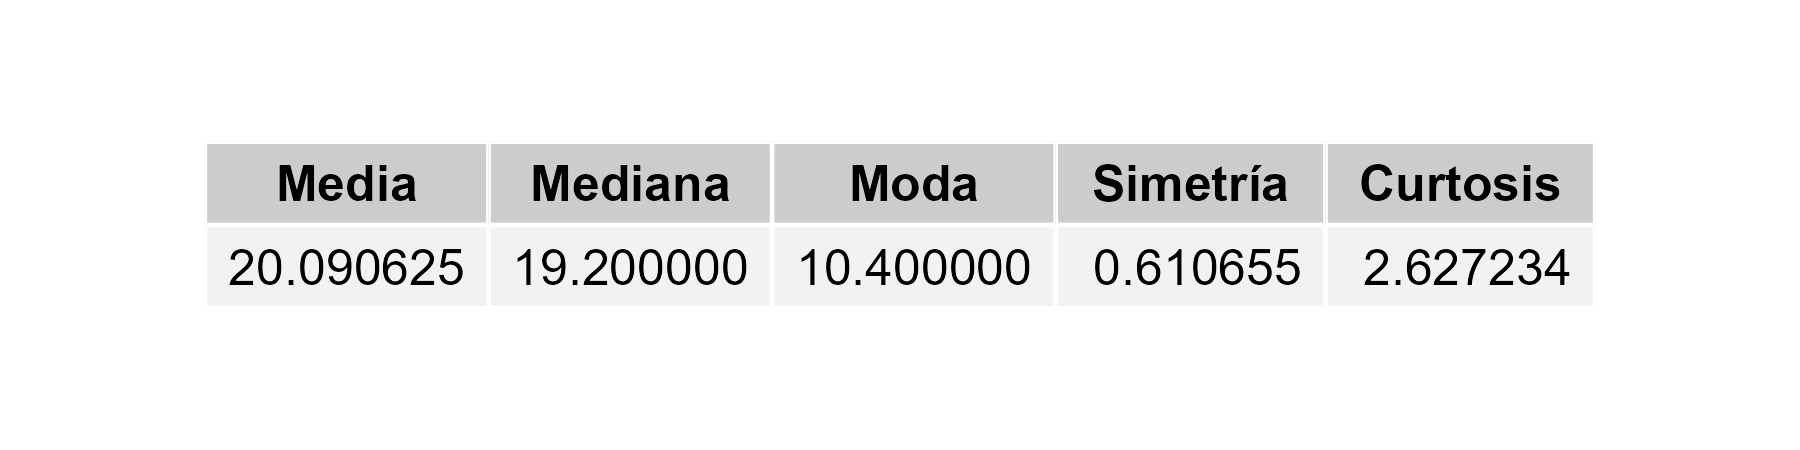
\includegraphics[width=0.8\textwidth]{MTC/mpg_central.png}
		      \caption{Medidas de tendencia central para la variable \texttt{mpg}.}
		      \label{fig:mpg_central}
	      \end{figure}

	      \begin{figure}[H]
		      \centering
		      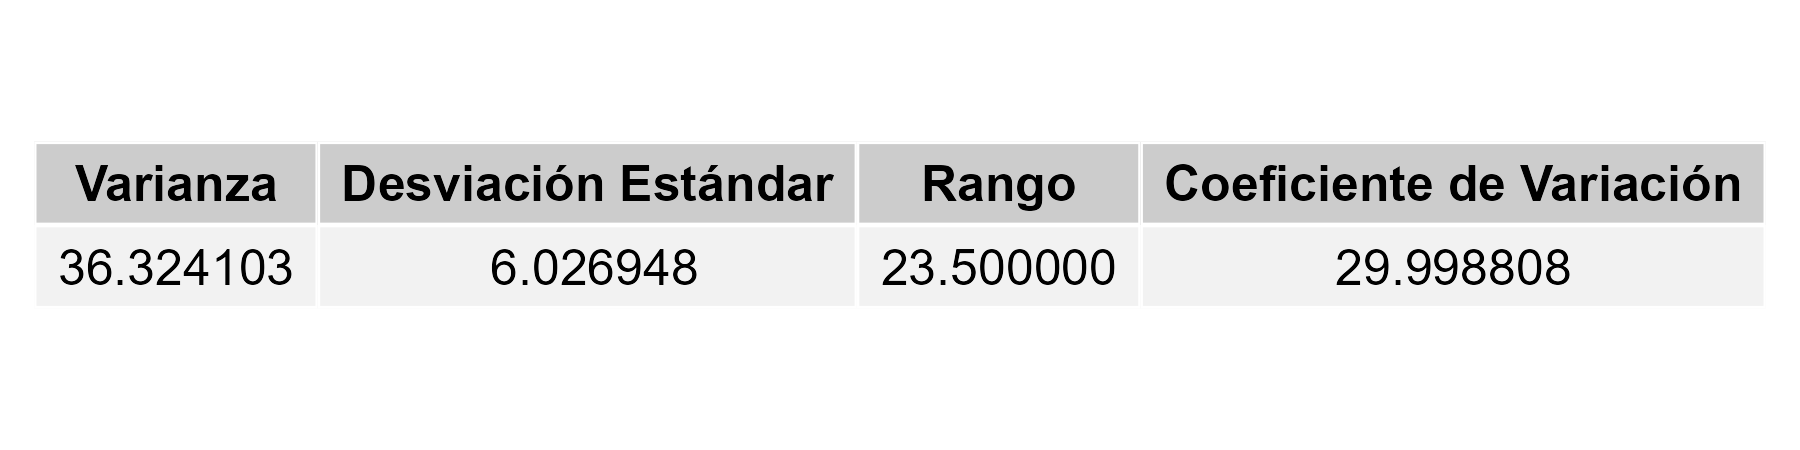
\includegraphics[width=0.8\textwidth]{MTC/mpg_dispersion.png}
		      \caption{Medidas de dispersión para la variable \texttt{mpg}.}
		      \label{fig:mpg_dispersion}
	      \end{figure} 
	  
	      \begin{itemize}
		      \item \textbf{Media:} El promedio de millas por galón es de 20.09. Este valor nos indica el rendimiento promedio de combustible de los vehículos analizados.
		      \item \textbf{Mediana:} El valor central es de 19.2 mpg, lo que implica que el 50\% de los vehículos tienen un rendimiento inferior o igual a este valor.
		      \item \textbf{Moda:} El valor que más se repite es 10.4 mpg, lo cual sugiere que un subconjunto de vehículos tiene un rendimiento significativamente bajo.
		      \item \textbf{Simetría:} Con un valor de 0.61, la distribución está sesgada positivamente, indicando que hay más valores bajos de mpg con algunos valores altos.
		      \item \textbf{Curtosis:} El valor de 2.63 indica que la distribución es leptocúrtica, con colas más pesadas que una distribución normal.
		      \item \textbf{Varianza y Desviación Estándar:} La varianza es 36.32 y la desviación estándar es 6.03, lo que revela una dispersión moderada alrededor de la media.
		      \item \textbf{Rango:} La diferencia entre el máximo y mínimo es de 23.5 mpg, mostrando una considerable variabilidad en el rendimiento.
		      \item \textbf{Coeficiente de Variación:} Con un 30\%, hay una variabilidad moderada en relación con la media.
	      \end{itemize}

		  \begin{figure}[H]
			\centering
			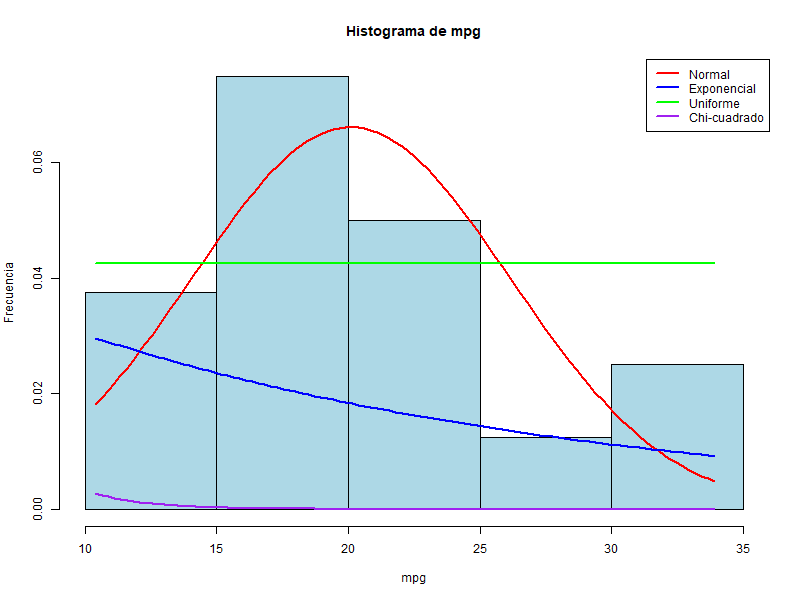
\includegraphics[width=0.5\textwidth]{Densidad/histograma_mpg.png}
			\caption{Histograma para mpg}
			\label{fig:histograma_mpg}
			\vspace{0.5cm}
		\end{figure}

	\item \textbf{cyl (Cylinders)}

	      \begin{itemize}
		      \item \textbf{Descripción:} Número de cilindros en el motor del automóvil.
		      \item \textbf{Escala:} Cuantitativa Discreta.
		      \item \textbf{Significado:} Indica cuántos cilindros tiene el motor. Generalmente, los valores comunes son 4, 6 u 8 cilindros.
	      \end{itemize}

	      \begin{figure}[H]
		      \centering
		      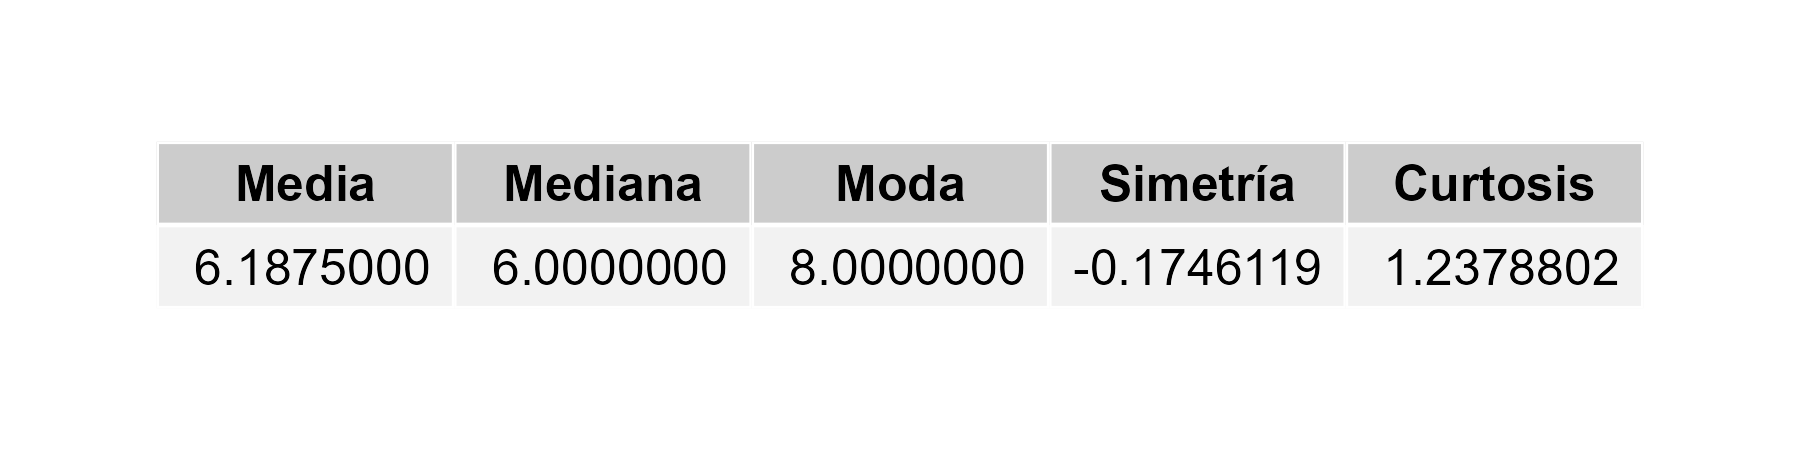
\includegraphics[width=0.8\textwidth]{MTC/cyl_central.png}
		      \caption{Medidas de tendencia central para la variable \texttt{cyl}.}
		      \label{fig:cyl_central}
	      \end{figure}

	      \begin{figure}[H]
		      \centering
		      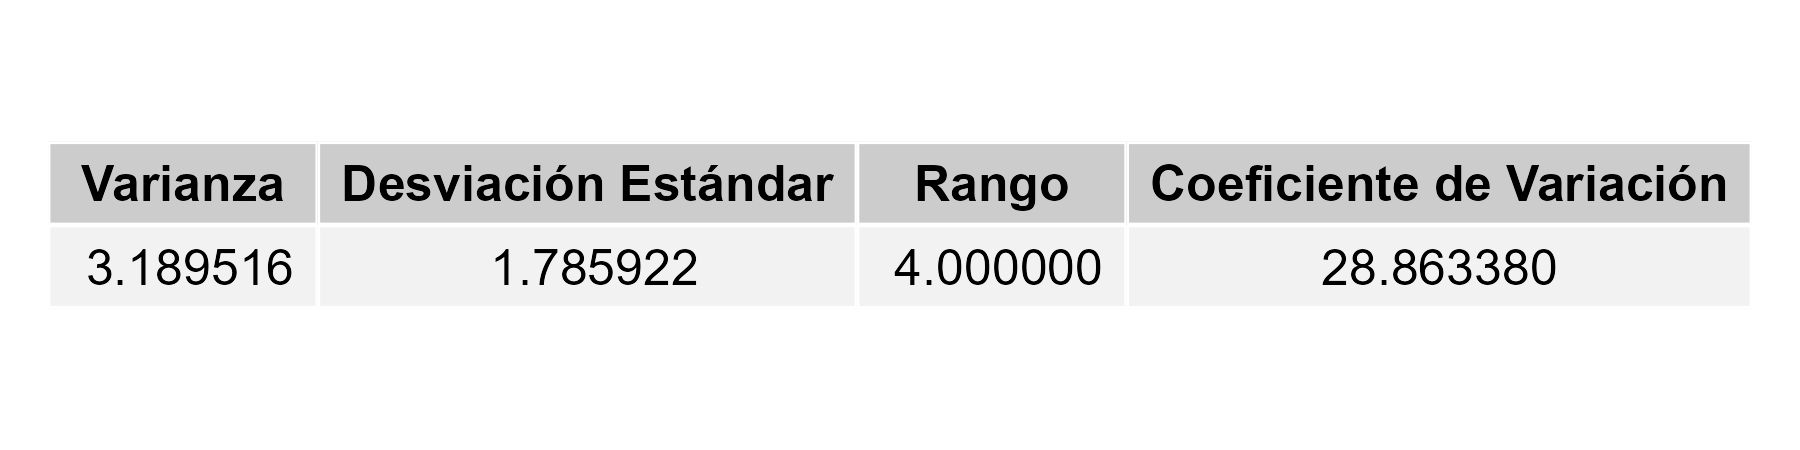
\includegraphics[width=0.8\textwidth]{MTC/cyl_dispersion.png}
		      \caption{Medidas de dispersión para la variable \texttt{cyl}.}
		      \label{fig:cyl_dispersion}
	      \end{figure}

	      \begin{itemize}
		      \item \textbf{Media:} El número promedio de cilindros es 6.19, indicando que la mayoría de los vehículos tienen entre 6 y 8 cilindros.
		      \item \textbf{Mediana:} El valor central es 6, lo que significa que la mitad de los autos tiene 6 cilindros o menos.
		      \item \textbf{Moda:} La moda es 8 cilindros, lo que sugiere que es el tipo más común en el conjunto de datos.
		      \item \textbf{Simetría:} Un valor de -0.17 indica una ligera asimetría negativa, donde algunos vehículos tienen menos cilindros de lo esperado.
		      \item \textbf{Curtosis:} Con 1.24, la distribución es platicúrtica, más plana que una normal.
		      \item \textbf{Varianza y Desviación Estándar:} La varianza es 3.19 y la desviación estándar es 1.79, sugiriendo una dispersión moderada.
		      \item \textbf{Rango:} El rango de 4 cilindros refleja una variabilidad moderada en la configuración del motor.
		      \item \textbf{Coeficiente de Variación:} Con 28.86\%, indica una moderada variabilidad relativa en el número de cilindros.
	      \end{itemize}

		  \begin{figure}[H]
			\centering
			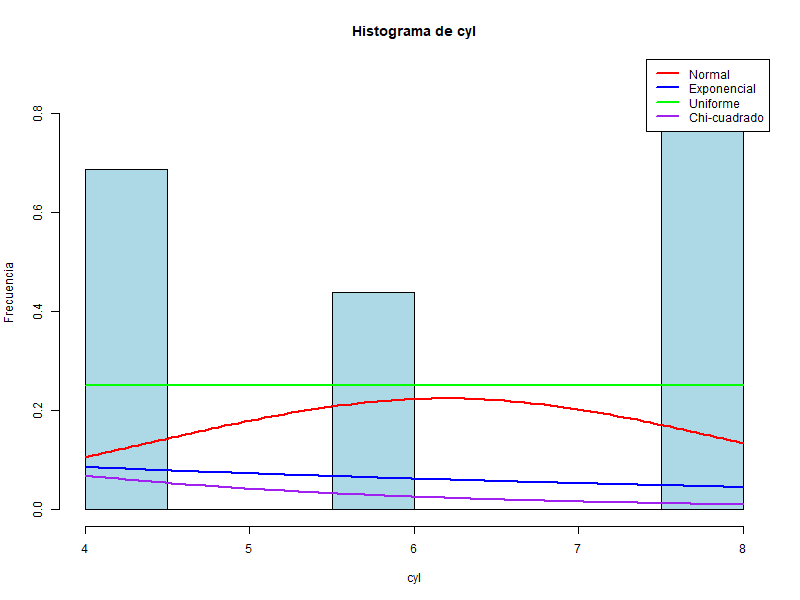
\includegraphics[width=0.5\textwidth]{Densidad/histograma_cyl.png}
			\caption{Histograma para cyl}
			\label{fig:histograma_cyl}
			\vspace{0.5cm}
		\end{figure}

	\item \textbf{disp (Displacement)}

	      \begin{itemize}
		      \item \textbf{Descripción:} Desplazamiento del motor en pulgadas cúbicas.
		      \item \textbf{Escala:} Cuantitativa Continua.
		      \item \textbf{Significado:} Es el volumen total desplazado por todos los pistones dentro del motor en una sola revolución. Es una medida del tamaño del motor.
	      \end{itemize}

	      \begin{figure}[H]
		      \centering
		      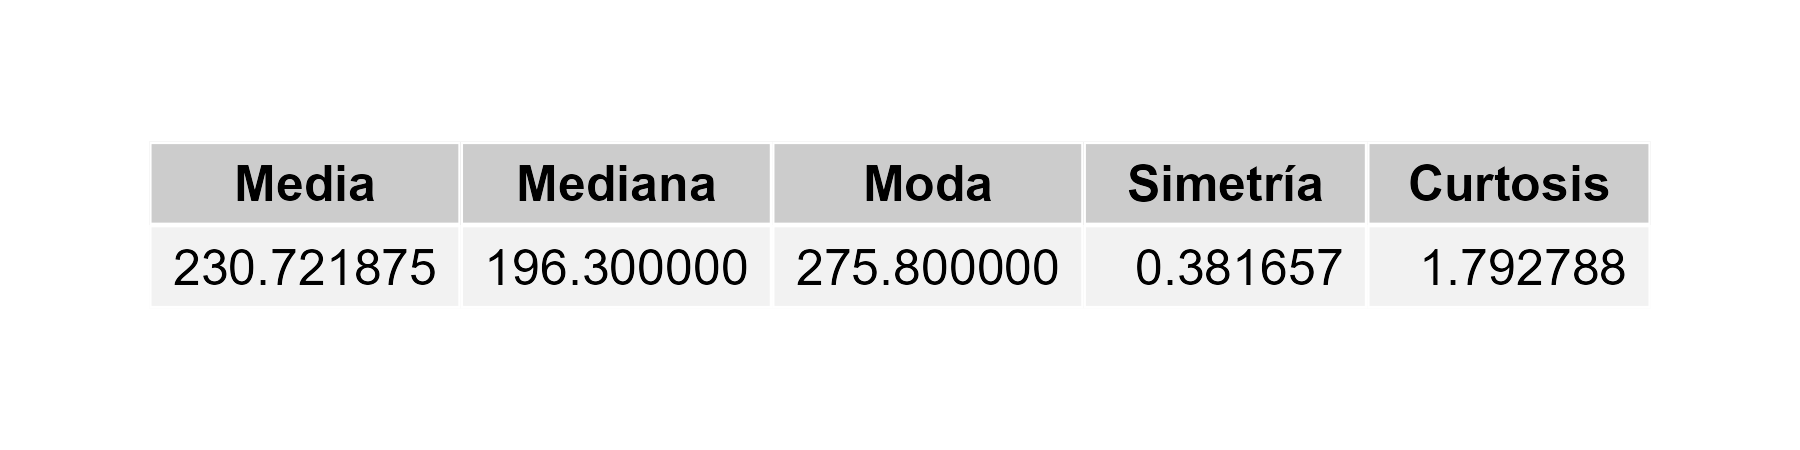
\includegraphics[width=0.8\textwidth]{MTC/disp_central.png}
		      \caption{Medidas de tendencia central para la variable \texttt{disp}.}
		      \label{fig:disp_central}
	      \end{figure}

	      \begin{figure}[H]
		      \centering
		      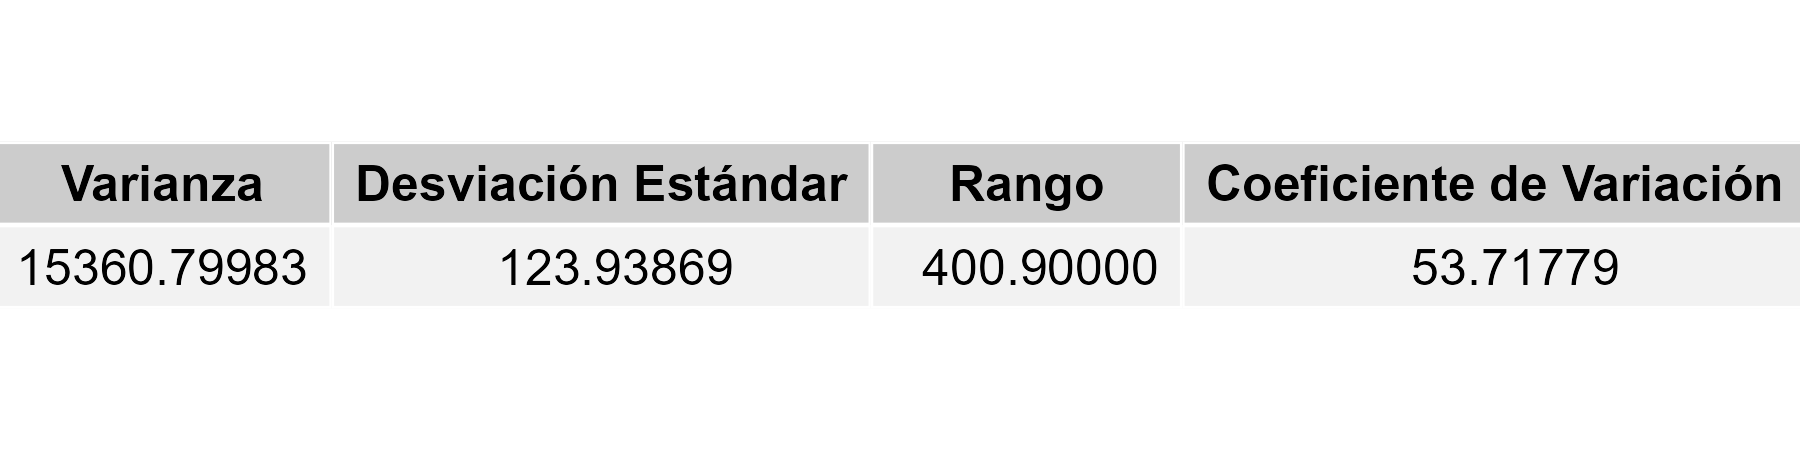
\includegraphics[width=0.8\textwidth]{MTC/disp_dispersion.png}
		      \caption{Medidas de dispersión para la variable \texttt{disp}.}
		      \label{fig:disp_dispersion}
	      \end{figure}

	      \begin{itemize}
		      \item \textbf{Media:} El promedio de desplazamiento es 230.72 pulgadas cúbicas, lo que refleja un tamaño del motor significativo en los vehículos.
		      \item \textbf{Mediana:} El valor central es 196.3, indicando que la mitad de los vehículos tiene un desplazamiento inferior a este.
		      \item \textbf{Moda:} La moda de 275.8 sugiere que algunos vehículos tienen un motor considerablemente grande.
		      \item \textbf{Simetría:} Un valor de 0.38 indica una ligera asimetría positiva, con algunos motores muy grandes que aumentan la media.
		      \item \textbf{Curtosis:} Con 1.79, la distribución es platicúrtica, indicando colas menos pesadas.
		      \item \textbf{Varianza y Desviación Estándar:} La alta varianza de 15360.80 y desviación estándar de 123.94 indican una gran dispersión.
		      \item \textbf{Rango:} El rango de 400.9 muestra una gran diferencia en el tamaño del motor entre los vehículos.
		      \item \textbf{Coeficiente de Variación:} Con un 53.72\%, existe una alta variabilidad relativa en el desplazamiento.
	      \end{itemize}

		  \begin{figure}[H]
			\centering
			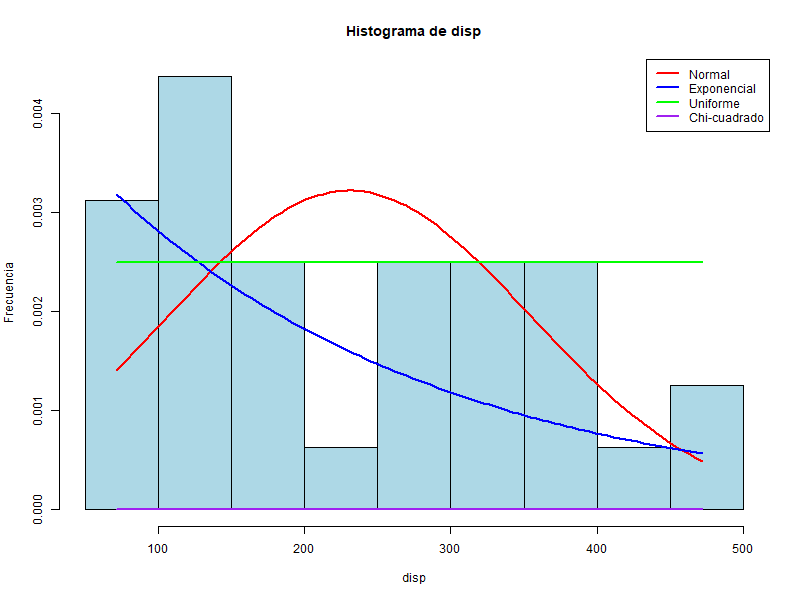
\includegraphics[width=0.5\textwidth]{Densidad/histograma_disp.png}
			\caption{Histograma para disp}
			\label{fig:histograma_disp}
			\vspace{0.5cm}
		\end{figure}

	\item \textbf{hp (Horsepower)}

	      \begin{itemize}
		      \item \textbf{Descripción:} Potencia del motor en caballos de fuerza.
		      \item \textbf{Escala:} Es una variable Cuantitativa que puede tener valores Continuos, pero en este caso solo guarda valores Discretos, por tanto la trataremos como Cuantitativa Discreta.
		      \item \textbf{Significado:} Mide la potencia del motor, es decir, la capacidad del motor para realizar trabajo en una unidad de tiempo.
	      \end{itemize}

	      \begin{figure}[H]
		      \centering
		      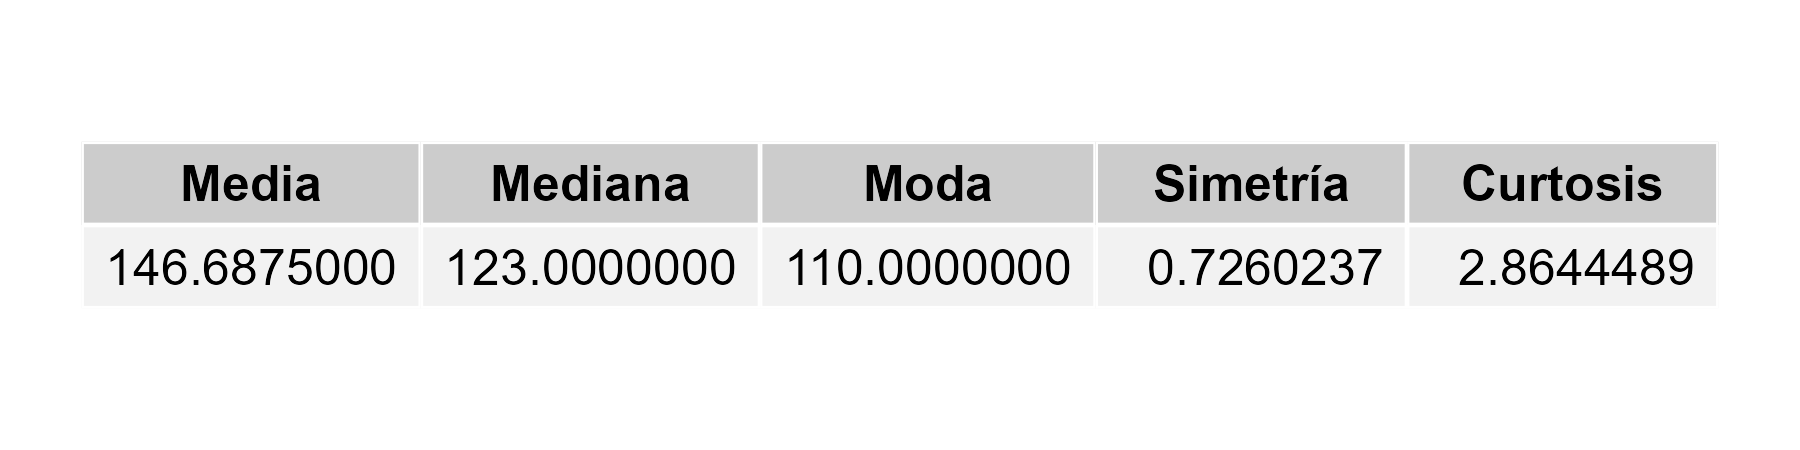
\includegraphics[width=0.8\textwidth]{MTC/hp_central.png}
		      \caption{Medidas de tendencia central para la variable \texttt{hp}.}
		      \label{fig:hp_central}
	      \end{figure}

	      \begin{figure}[H]
		      \centering
		      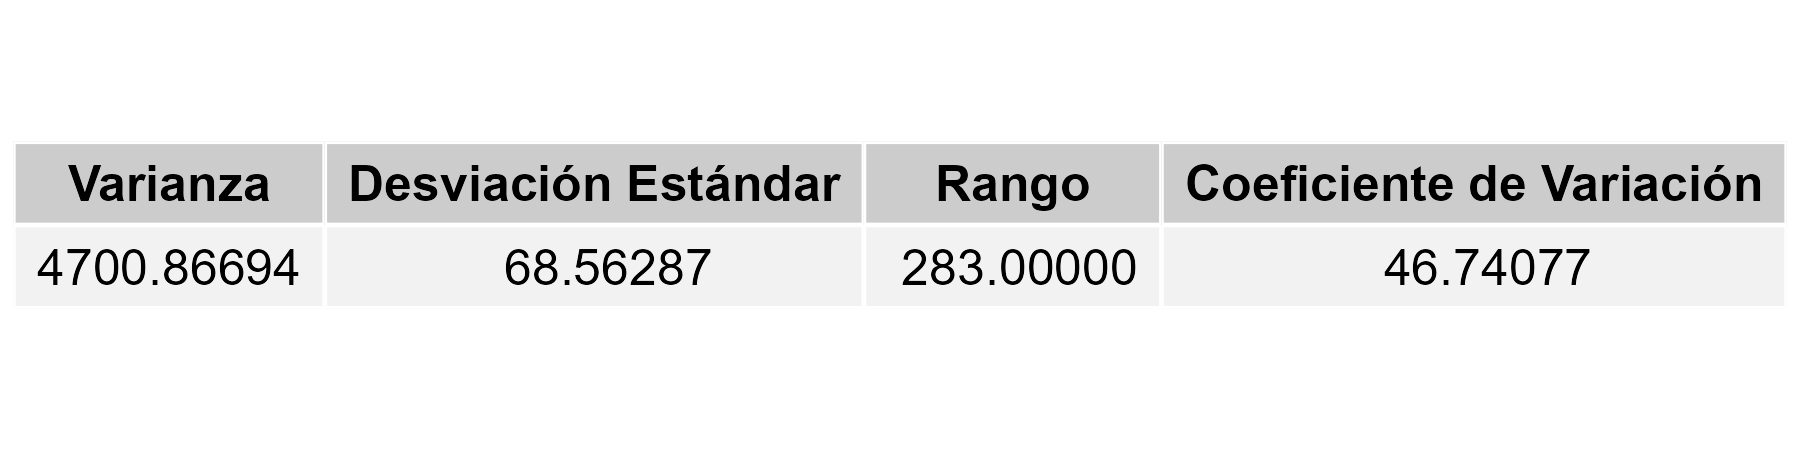
\includegraphics[width=0.8\textwidth]{MTC/hp_dispersion.png}
		      \caption{Medidas de dispersión para la variable \texttt{hp}.}
		      \label{fig:hp_dispersion}
	      \end{figure}

	      \begin{itemize}
		      \item \textbf{Media:} El promedio es 146.69 caballos de fuerza, reflejando una potencia moderada en los vehículos.
		      \item \textbf{Mediana:} Con 123 hp, la mitad de los vehículos tiene menos potencia que este valor.
		      \item \textbf{Moda:} La moda es 110 hp, común en vehículos de potencia media.
		      \item \textbf{Simetría:} Un valor de 0.73 indica una asimetría positiva, sugiriendo que algunos autos tienen potencia mucho mayor que la media.
		      \item \textbf{Curtosis:} El valor de 2.86 indica colas más pesadas, sugiriendo algunos valores extremos de potencia.
		      \item \textbf{Varianza y Desviación Estándar:} La varianza es 4700.87 y la desviación estándar 68.56, lo que indica una alta dispersión en la potencia.
		      \item \textbf{Rango:} El rango de 283 hp muestra una diferencia significativa entre los autos menos y más potentes.
		      \item \textbf{Coeficiente de Variación:} Un 46.74\% indica una alta variabilidad relativa.
	      \end{itemize}

		  \begin{figure}[H]
			\centering
			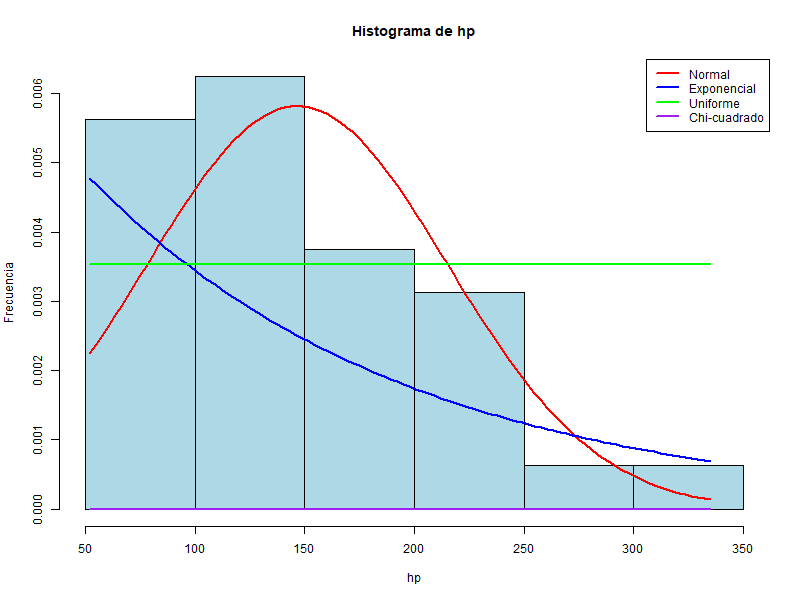
\includegraphics[width=0.5\textwidth]{Densidad/histograma_hp.png}
			\caption{Histograma para hp}
			\label{fig:histograma_hp}
			\vspace{0.5cm}
		\end{figure}

	\item \textbf{drat (Rear Axle Ratio)}

	      \begin{itemize}
		      \item \textbf{Descripción:} Relación de transmisión del eje trasero.
		      \item \textbf{Escala:} Cuantitativa Continua.
		      \item \textbf{Significado:} Es la relación entre las revoluciones del eje de transmisión y las revoluciones del eje trasero. Afecta el rendimiento y la velocidad del vehículo.
	      \end{itemize}

	      \begin{figure}[H]
		      \centering
		      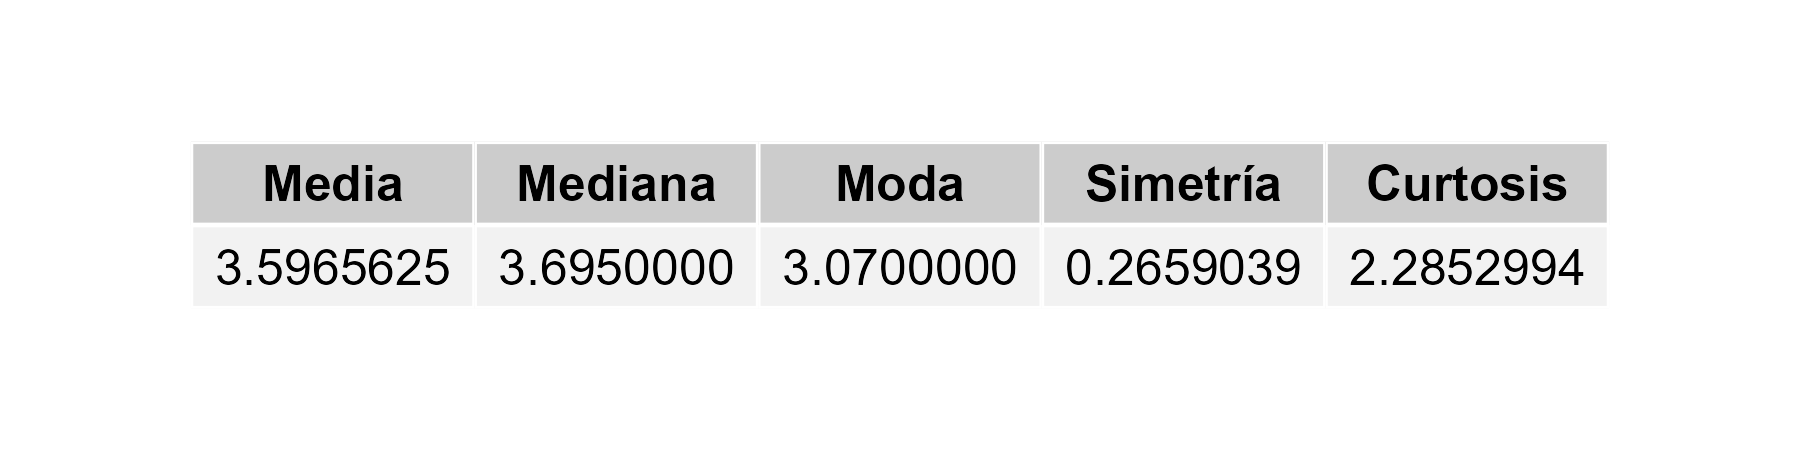
\includegraphics[width=0.8\textwidth]{MTC/drat_central.png}
		      \caption{Medidas de tendencia central para la variable \texttt{drat}.}
		      \label{fig:drat_central}
	      \end{figure}

	      \begin{figure}[H]
		      \centering
		      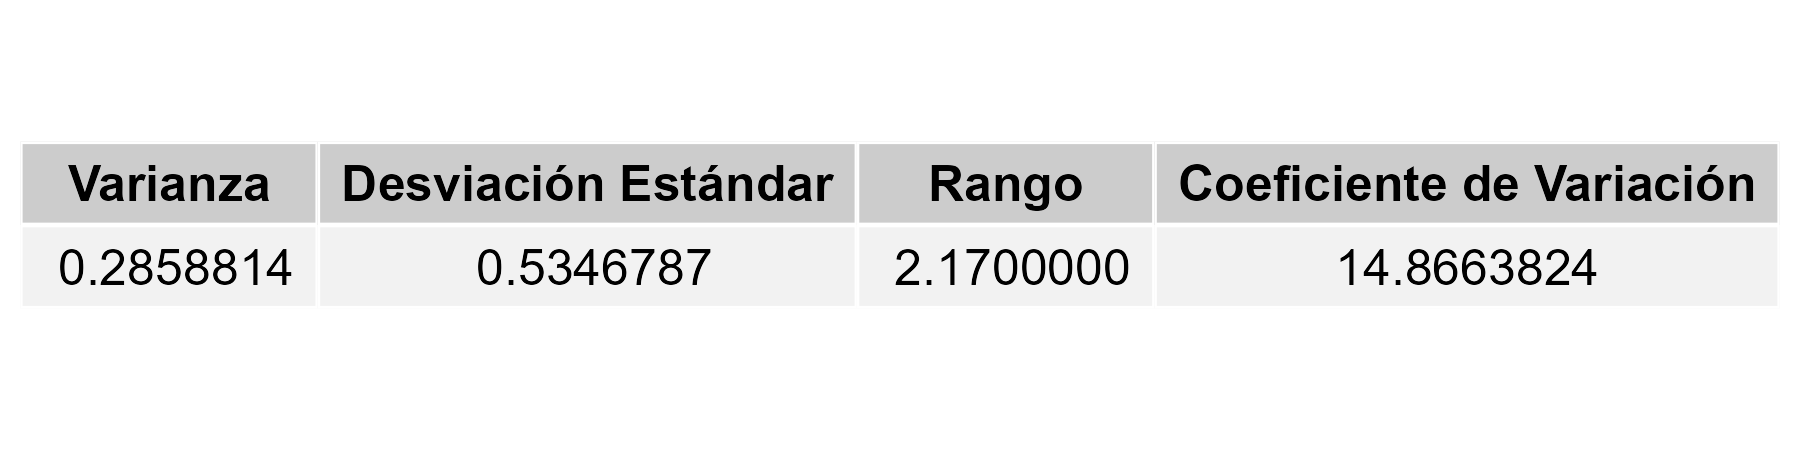
\includegraphics[width=0.8\textwidth]{MTC/drat_dispersion.png}
		      \caption{Medidas de dispersión para la variable \texttt{drat}.}
		      \label{fig:drat_dispersion}
	      \end{figure}
	     
	      \begin{itemize}
		      \item \textbf{Media:} La relación promedio es 3.60, reflejando las configuraciones de transmisión en los vehículos.
		      \item \textbf{Mediana:} Con 3.70, la mitad de las relaciones del eje están por debajo de este valor.
		      \item \textbf{Moda:} El valor más común es 3.07.
		      \item \textbf{Simetría:} Un valor de 0.27 sugiere una ligera asimetría positiva.
		      \item \textbf{Curtosis:} Con 2.29, la distribución es mesocúrtica, cercana a la normal.
		      \item \textbf{Varianza y Desviación Estándar:} La baja varianza de 0.29 y desviación estándar de 0.53 indican poca dispersión.
		      \item \textbf{Rango:} Un rango de 2.17 muestra cierta variabilidad en las relaciones del eje.
		      \item \textbf{Coeficiente de Variación:} El 14.87\% sugiere baja variabilidad relativa.
	      \end{itemize}

		  \begin{figure}[H]
			\centering
			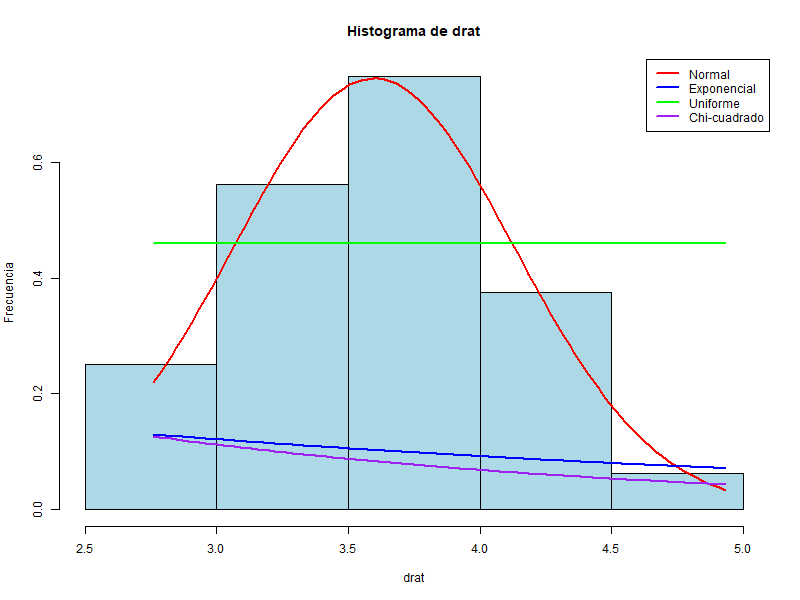
\includegraphics[width=0.5\textwidth]{Densidad/histograma_drat.png}
			\caption{Histograma para drat}
			\label{fig:histograma_drat}
			\vspace{0.5cm}
		\end{figure}

	\item \textbf{wt (Weight)}

	      \begin{itemize}
		      \item \textbf{Descripción:} Peso del automóvil en miles de libras.
		      \item \textbf{Escala:} Cuantitativa Continua.
		      \item \textbf{Significado:} El peso del automóvil influye en su eficiencia, aceleración y manejo.
	      \end{itemize}

	      \begin{figure}[H]
		      \centering
		      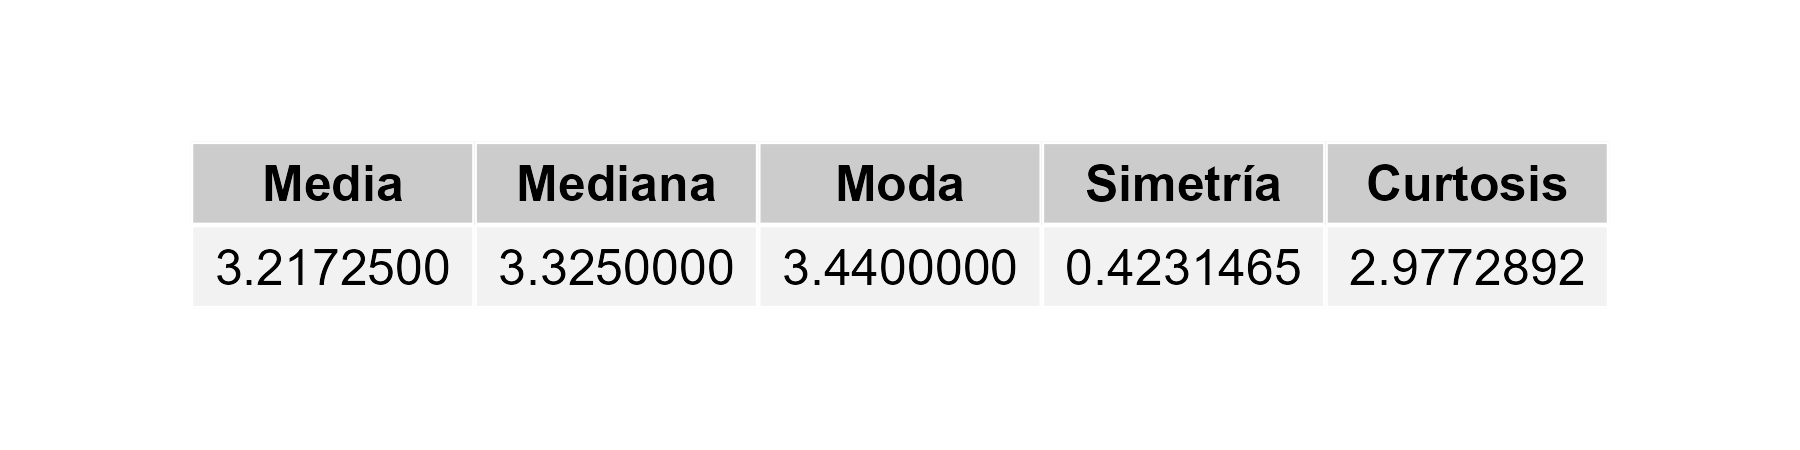
\includegraphics[width=0.8\textwidth]{MTC/wt_central.png}
		      \caption{Medidas de tendencia central para la variable \texttt{wt}.}
		      \label{fig:wt_central}
	      \end{figure}

	      \begin{figure}[H]
		      \centering
		      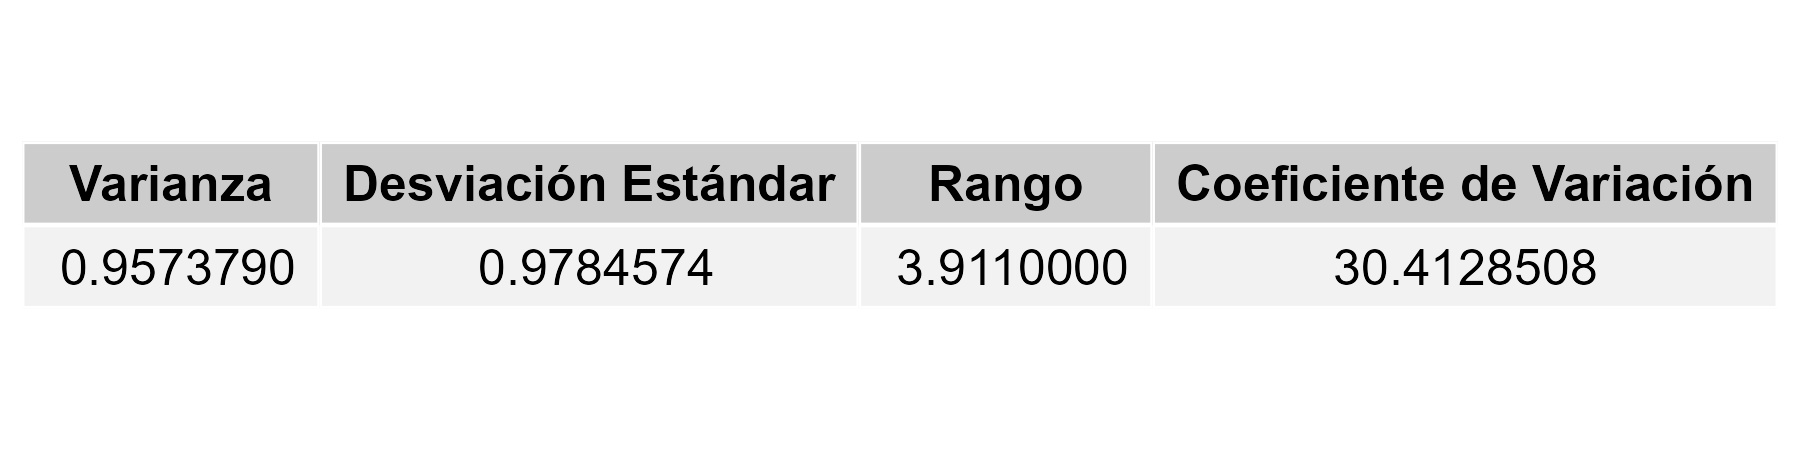
\includegraphics[width=0.8\textwidth]{MTC/wt_dispersion.png}
		      \caption{Medidas de dispersión para la variable \texttt{wt}.}
		      \label{fig:wt_dispersion}
	      \end{figure}
	    
	      \begin{itemize}
		      \item \textbf{Media:} El peso promedio es 3.22 (en miles de libras), reflejando el peso general de los vehículos.
		      \item \textbf{Mediana:} El valor central es 3.33.
		      \item \textbf{Moda:} La moda es 3.44, indicando que es un peso común entre los vehículos.
		      \item \textbf{Simetría:} Un valor de 0.42 sugiere una ligera asimetría positiva.
		      \item \textbf{Curtosis:} Con 2.98, la distribución es leptocúrtica.
		      \item \textbf{Varianza y Desviación Estándar:} La varianza de 0.96 y desviación estándar de 0.98 indican una moderada dispersión.
		      \item \textbf{Rango:} Un rango de 3.91 refleja una diferencia considerable en el peso de los vehículos.
		      \item \textbf{Coeficiente de Variación:} Con 30.41\%, hay una variabilidad moderada en relación a la media.
	      \end{itemize}

		  \begin{figure}[H]
			\centering
			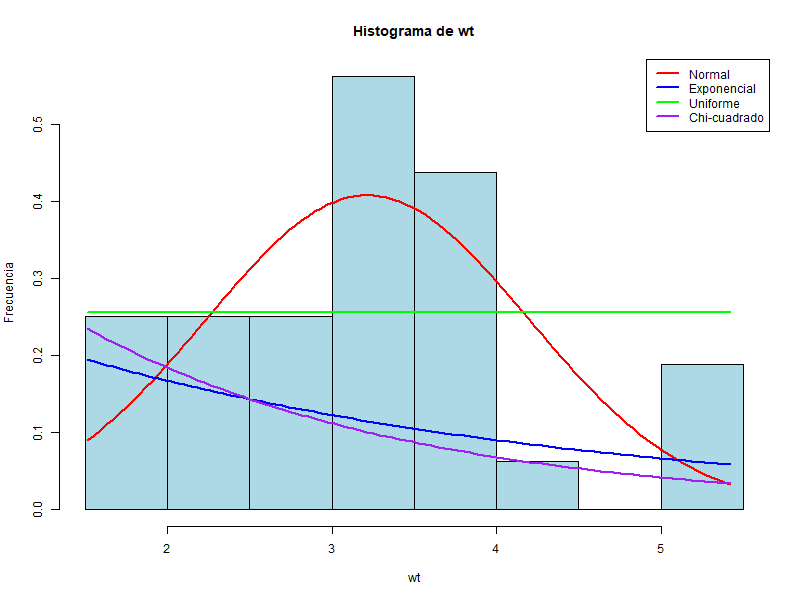
\includegraphics[width=0.5\textwidth]{Densidad/histograma_wt.png}
			\caption{Histograma para wt}
			\label{fig:histograma_wt}
			\vspace{0.5cm}
		\end{figure}

	\item \textbf{qsec (1/4 Mile Time)}

	      \begin{itemize}
		      \item \textbf{Descripción:} Tiempo en segundos para recorrer un cuarto de milla.
		      \item \textbf{Escala:} Cuantitativa Continua.
		      \item \textbf{Significado:} Es una medida del tiempo que tarda el automóvil en recorrer un cuarto de milla, comúnmente usado para medir el rendimiento en aceleración.
	      \end{itemize}

	      \begin{figure}[H]
		      \centering
		      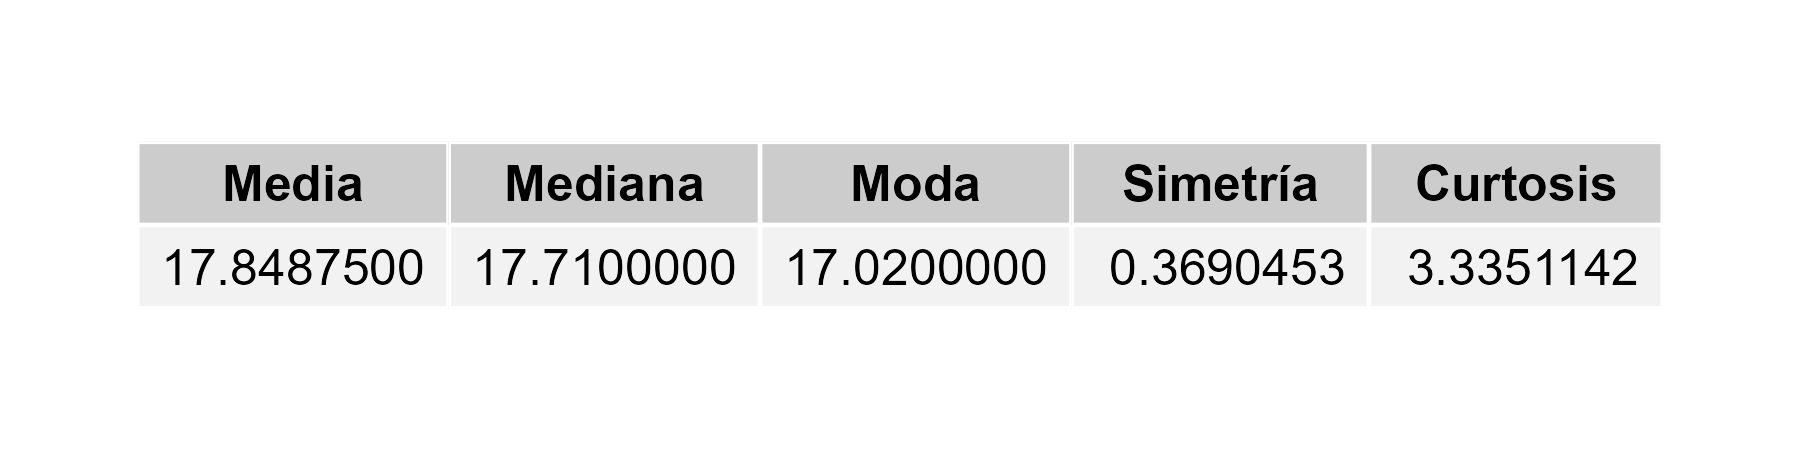
\includegraphics[width=0.8\textwidth]{MTC/qsec_central.png}
		      \caption{Medidas de tendencia central para la variable \texttt{qsec}.}
		      \label{fig:qsec_central}
	      \end{figure}

	      \begin{figure}[H]
		      \centering
		      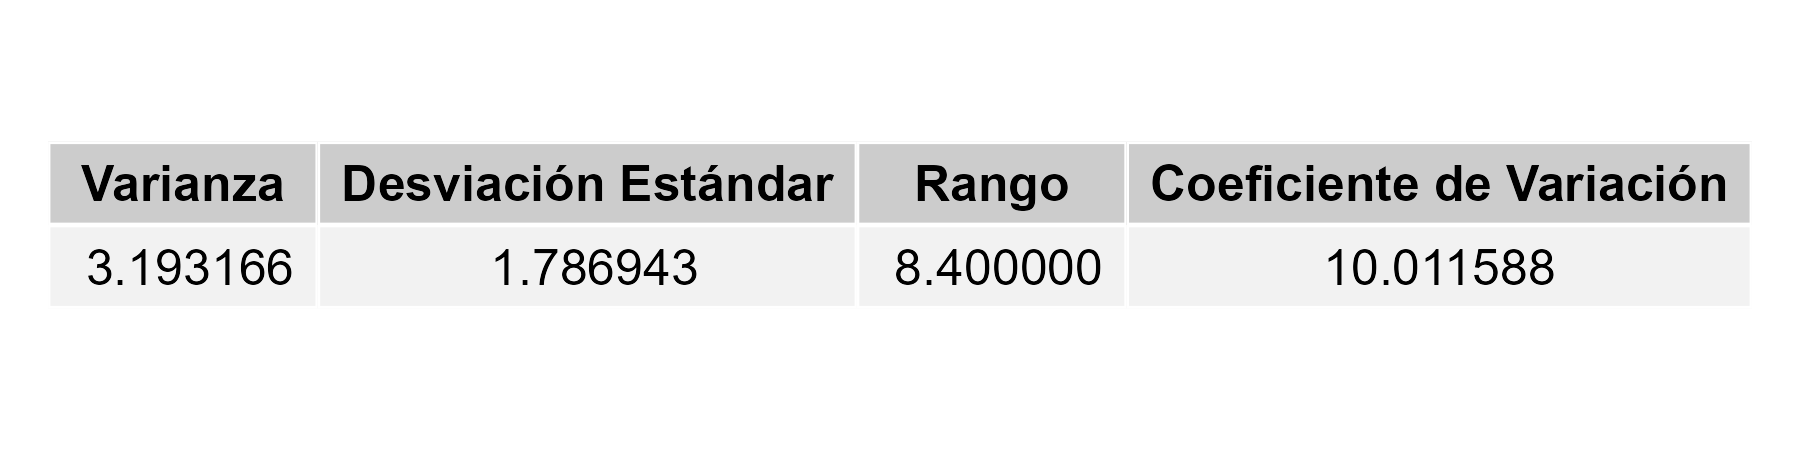
\includegraphics[width=0.8\textwidth]{MTC/qsec_dispersion.png}
		      \caption{Medidas de dispersión para la variable \texttt{qsec}.}
		      \label{fig:qsec_dispersion}
	      \end{figure}

	     
	      \begin{itemize}
		      \item \textbf{Media:} El promedio es 17.85 segundos, indicando el tiempo medio que tardan los vehículos en recorrer un cuarto de milla.
		      \item \textbf{Mediana:} El valor central es 17.71 segundos.
		      \item \textbf{Moda:} La moda es 17.02 segundos.
		      \item \textbf{Simetría:} Un valor de 0.37 indica una ligera asimetría positiva.
		      \item \textbf{Curtosis:} Con 3.34, la distribución es leptocúrtica.
		      \item \textbf{Varianza y Desviación Estándar:} La varianza es 3.19 y la desviación estándar es 1.79, lo que indica una dispersión moderada.
		      \item \textbf{Rango:} El rango de 8.4 segundos muestra variabilidad en la aceleración de los vehículos.
		      \item \textbf{Coeficiente de Variación:} Con un 10.01\%, hay poca variabilidad relativa.
	      \end{itemize}

		  \begin{figure}[H]
			\centering
			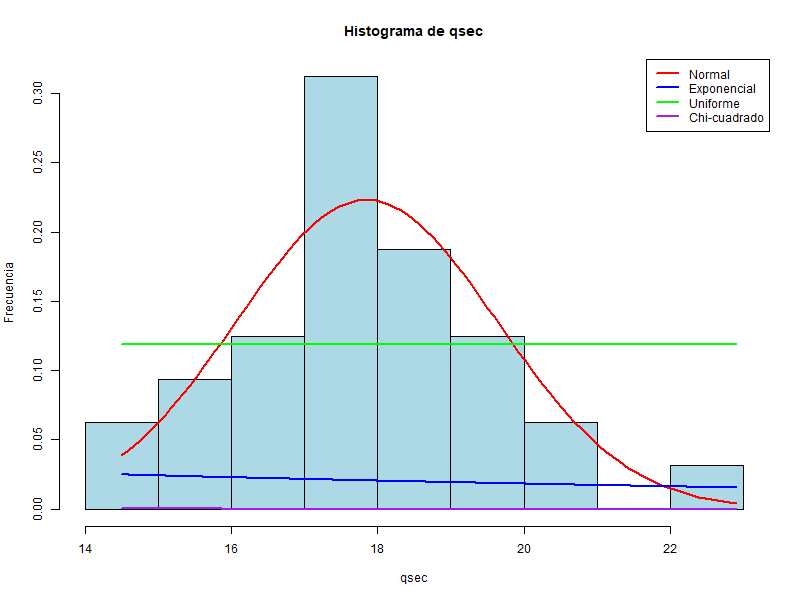
\includegraphics[width=0.5\textwidth]{Densidad/histograma_qsec.png}
			\caption{Histograma para qsec}
			\label{fig:histograma_qsec}
			\vspace{0.5cm}
		\end{figure}

	\item \textbf{vs (Engine Shape)}

	      \begin{itemize}
		      \item \textbf{Descripción:} Forma del motor (0 = motor en V, 1 = motor en línea).
		      \item \textbf{Escala:}  Esta es de cierta manera una variable cualitativa nominal, lo que esta convertida a Cuantitativa Discreta (Binaria).
		      \item \textbf{Significado:} Indica el tipo de configuración del motor: si los cilindros están dispuestos en forma de V o en línea.
	      \end{itemize}


	      \begin{figure}[H]
		      \centering
		      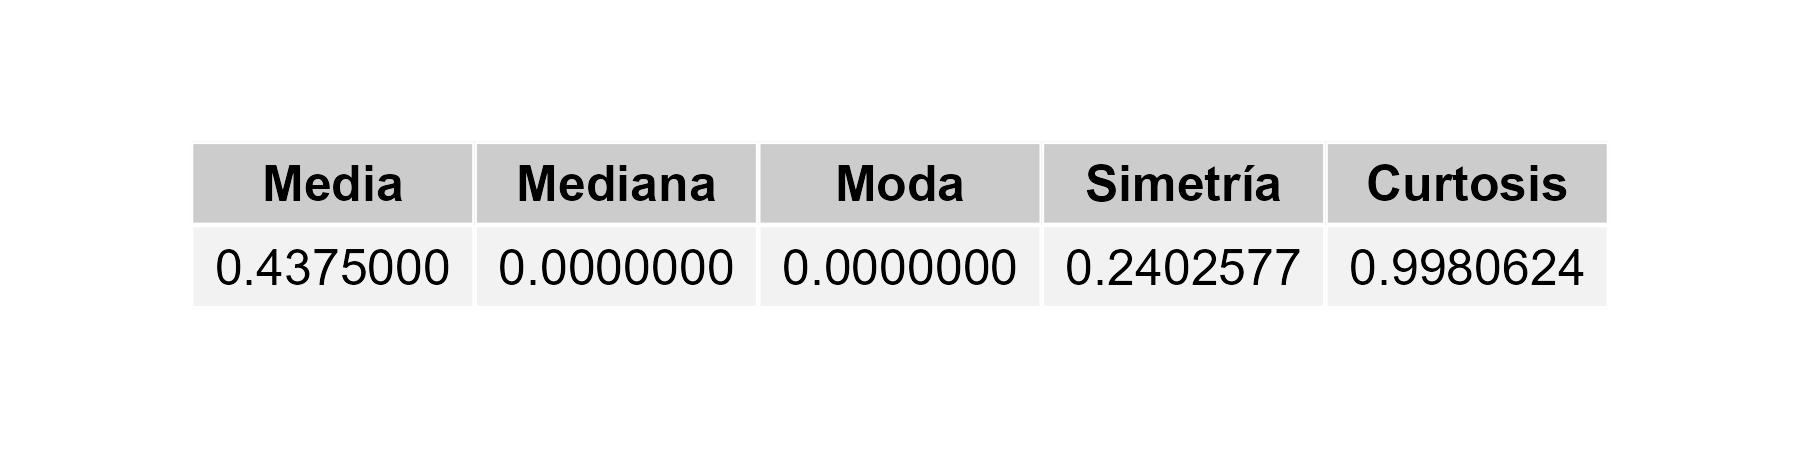
\includegraphics[width=0.8\textwidth]{MTC/vs_central.png}
		      \caption{Medidas de tendencia central para la variable \texttt{vs}.}
		      \label{fig:vs_central}
	      \end{figure}

	      \begin{figure}[H]
		      \centering
		      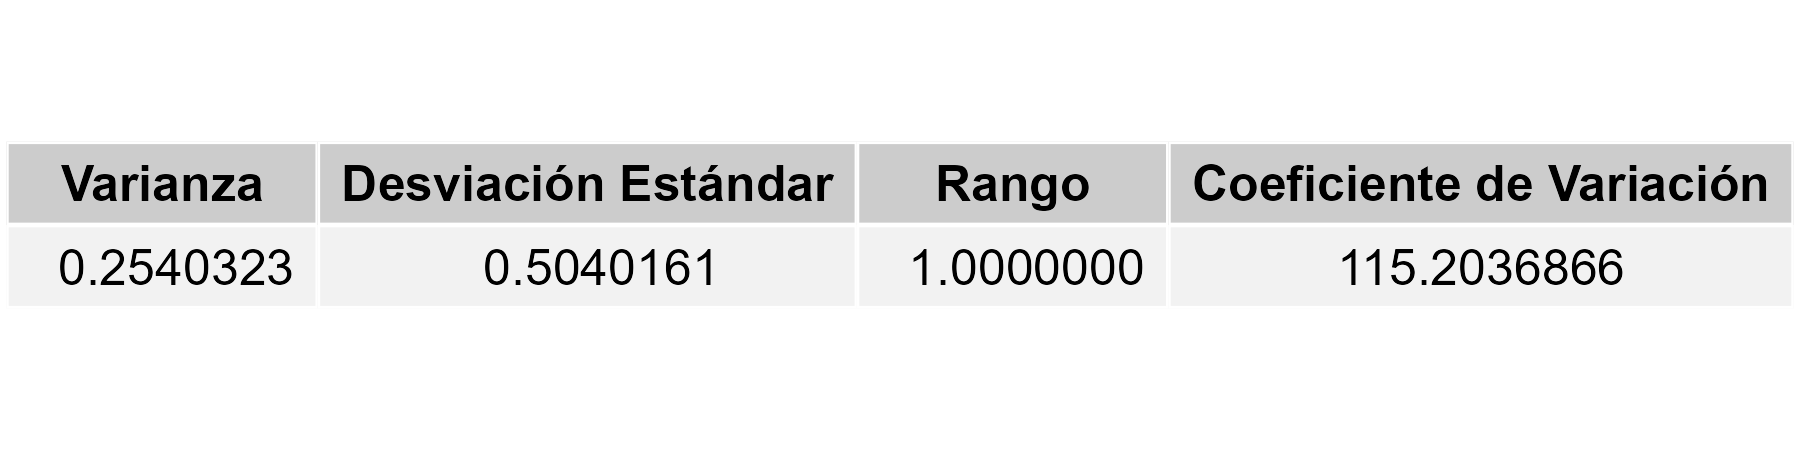
\includegraphics[width=0.8\textwidth]{MTC/vs_dispersion.png}
		      \caption{Medidas de dispersión para la variable \texttt{vs}.}
		      \label{fig:vs_dispersion}
	      \end{figure}
	    
	      \begin{itemize}
		      \item \textbf{Media:} El promedio es 0.44, lo que sugiere que aproximadamente el 44\% de los vehículos tienen un motor en línea.
		      \item \textbf{Mediana:} La mediana es 0, lo que significa que la mayoría de los vehículos tienen motores en V.
		      \item \textbf{Moda:} La moda es 0, reforzando que la configuración de motor en V es la más común.
		      \item \textbf{Simetría:} Un valor de 0.24 indica una ligera asimetría positiva.
		      \item \textbf{Curtosis:} Con 0.99, la distribución es casi mesocúrtica.
		      \item \textbf{Varianza y Desviación Estándar:} La varianza es 0.25 y la desviación estándar es 0.50, indicando poca dispersión.
		      \item \textbf{Rango:} El rango es 1, mostrando la variabilidad binaria.
		      \item \textbf{Coeficiente de Variación:} Con 115.20\%, existe una alta variabilidad relativa en esta variable binaria.
	      \end{itemize}

		  \begin{figure}[H]
			\centering
			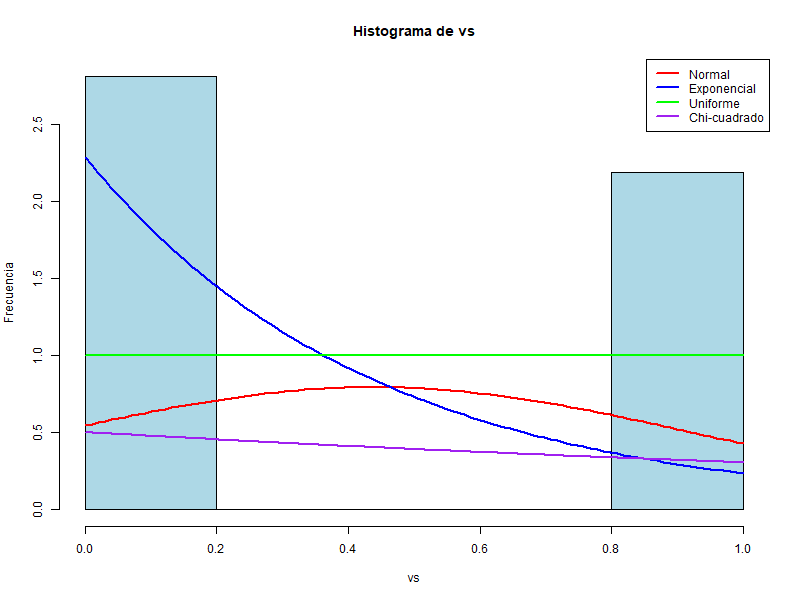
\includegraphics[width=0.5\textwidth]{Densidad/histograma_vs.png}
			\caption{Histograma para vs}
			\label{fig:histograma_vs}
			\vspace{0.5cm}
		\end{figure}

	\item \textbf{am (Transmission)}

	      \begin{itemize}
		      \item \textbf{Descripción:} Tipo de transmisión (0 = automática, 1 = manual).
		      \item \textbf{Escala:} Esta es de cierta manera una variable cualitativa nominal, lo que esta convertida a CUantitativa Discreta (Binaria).
		      \item \textbf{Significado:} Indica si el automóvil tiene una transmisión automática o manual.
	      \end{itemize}

	      \begin{figure}[H]
		      \centering
		      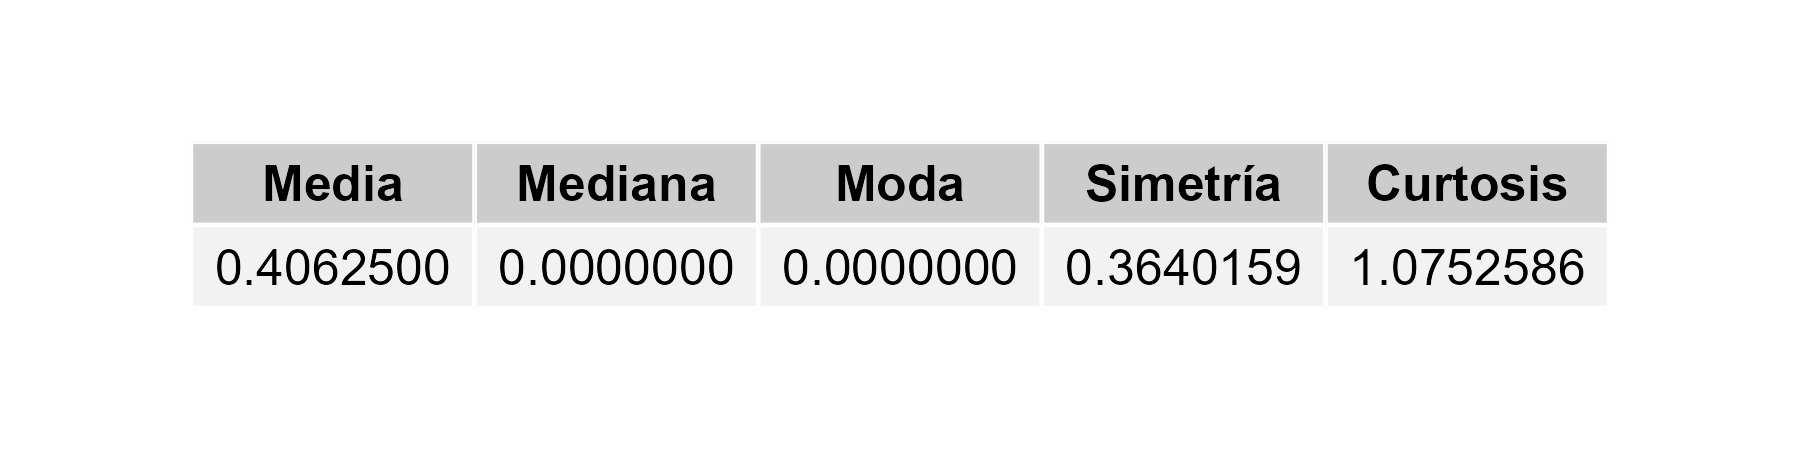
\includegraphics[width=0.8\textwidth]{MTC/am_central.png}
		      \caption{Medidas de tendencia central para la variable \texttt{am}.}
		      \label{fig:am_central}
	      \end{figure}

	      \begin{figure}[H]
		      \centering
		      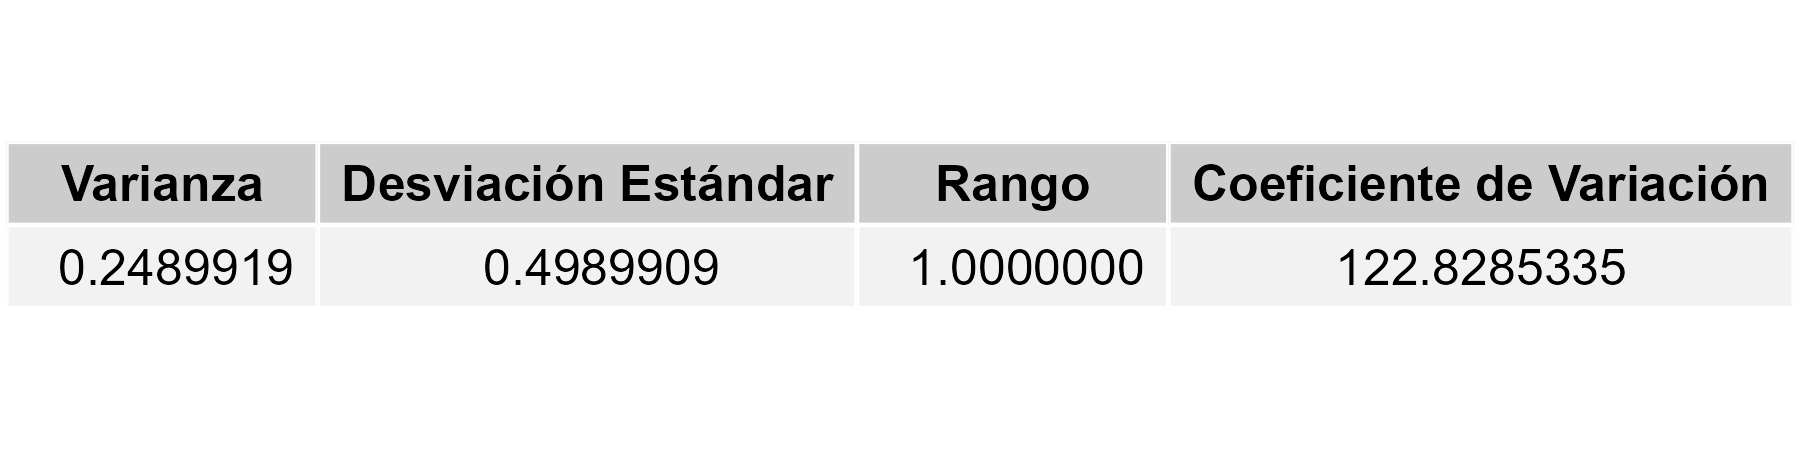
\includegraphics[width=0.8\textwidth]{MTC/am_dispersion.png}
		      \caption{Medidas de dispersión para la variable \texttt{am}.}
		      \label{fig:am_dispersion}
	      \end{figure}
	     
	      \begin{itemize}
		      \item \textbf{Media:} El promedio es 0.41, indicando que aproximadamente el 41\% de los vehículos tienen transmisión manual.
		      \item \textbf{Mediana:} El valor central es 0, indicando que la mayoría de los vehículos tienen transmisión automática.
		      \item \textbf{Moda:} La moda es 0, reforzando que la configuración automática es la más común.
		      \item \textbf{Simetría:} Un valor de 0.36 indica una ligera asimetría positiva.
		      \item \textbf{Curtosis:} Con 1.08, la distribución es bastante plana.
		      \item \textbf{Varianza y Desviación Estándar:} La varianza de 0.25 y desviación estándar de 0.50 indican poca dispersión.
		      \item \textbf{Rango:} Un rango de 1 refleja la variabilidad binaria.
		      \item \textbf{Coeficiente de Variación:} Con 122.83\%, hay una alta variabilidad relativa.
	      \end{itemize}

		  \begin{figure}[H]
			\centering
			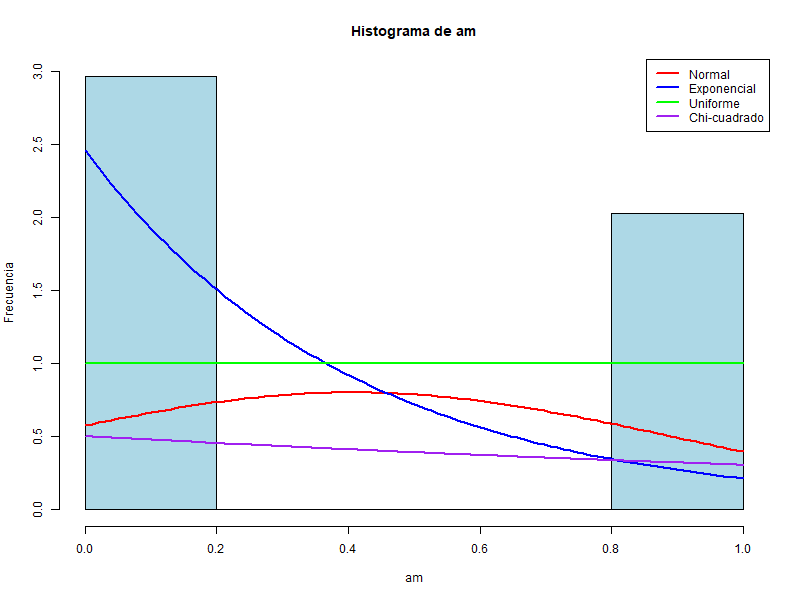
\includegraphics[width=0.5\textwidth]{Densidad/histograma_am.png}
			\caption{Histograma para am}
			\label{fig:histograma_am}
			\vspace{0.5cm} % Espacio entre las imágenes
		\end{figure}

	\item \textbf{gear (Gears)}

	      \begin{itemize}
		      \item \textbf{Descripción:} Número de velocidades de la caja de cambios.
		      \item \textbf{Escala:} Cuantitativa Discreta.
		      \item \textbf{Significado:} Indica cuántas marchas tiene la caja de cambios del automóvil.
	      \end{itemize}

	      \begin{figure}[H]
		      \centering
		      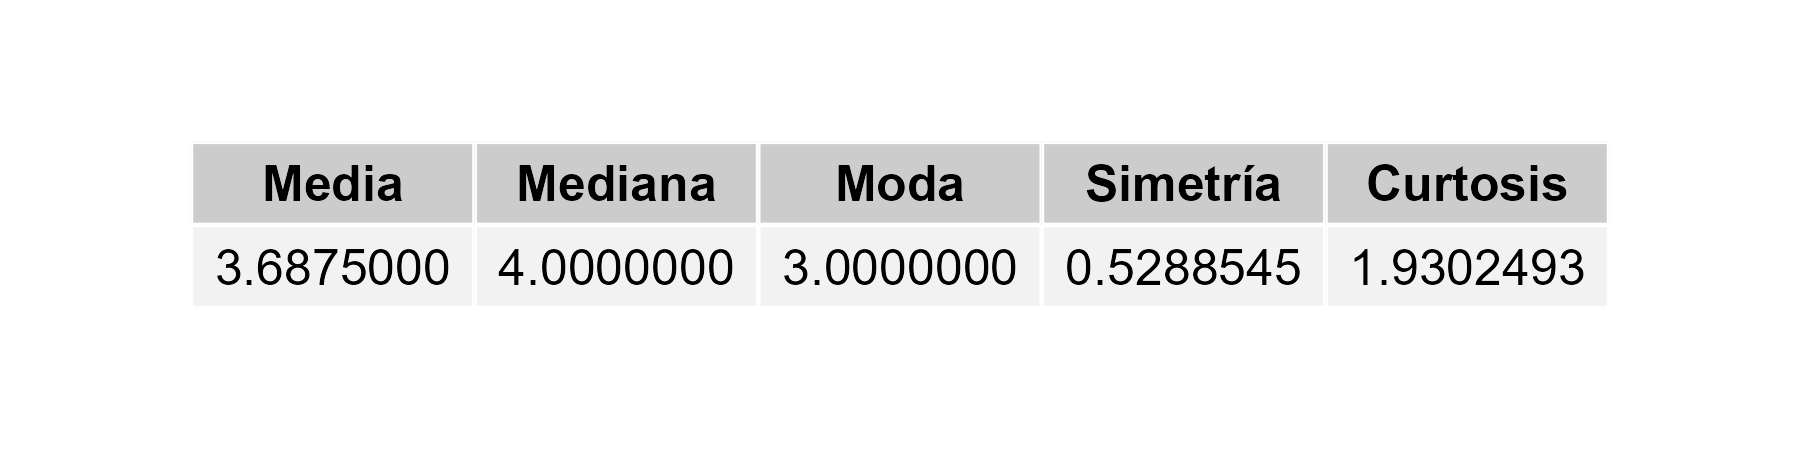
\includegraphics[width=0.8\textwidth]{MTC/gear_central.png}
		      \caption{Medidas de tendencia central para la variable \texttt{gear}.}
		      \label{fig:gear_central}
	      \end{figure}

	      \begin{figure}[H]
		      \centering
		      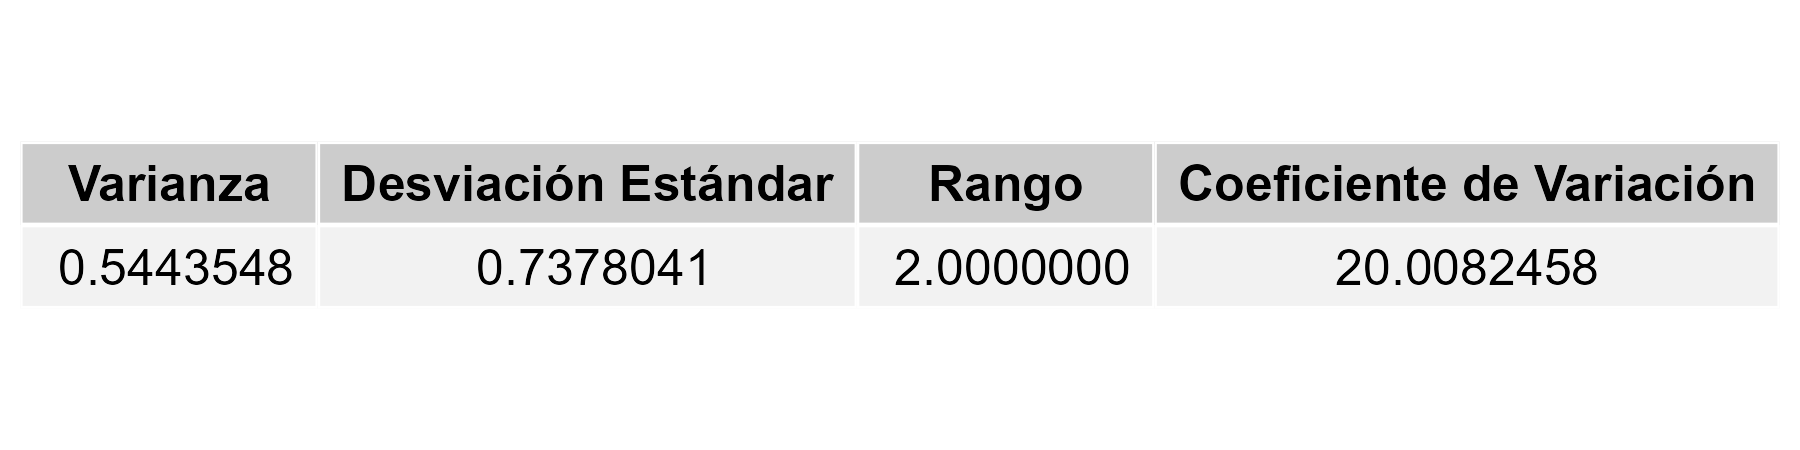
\includegraphics[width=0.8\textwidth]{MTC/gear_dispersion.png}
		      \caption{Medidas de dispersión para la variable \texttt{gear}.}
		      \label{fig:gear_dispersion}
	      \end{figure}
	      
	      \begin{itemize}
		      \item \textbf{Media:} El promedio es 3.69, indicando un predominio de autos con 3 a 4 marchas.
		      \item \textbf{Mediana:} El valor central es 4 marchas.
		      \item \textbf{Moda:} La moda es 3 marchas, lo que sugiere que es la configuración más común.
		      \item \textbf{Simetría:} Un valor de 0.53 indica una asimetría positiva, con algunos vehículos que tienen más marchas.
		      \item \textbf{Curtosis:} Con 1.93, la distribución es mesocúrtica.
		      \item \textbf{Varianza y Desviación Estándar:} La varianza de 0.54 y desviación estándar de 0.74 sugieren dispersión moderada.
		      \item \textbf{Rango:} El rango de 2 marchas muestra cierta variabilidad en el número de marchas.
		      \item \textbf{Coeficiente de Variación:} Con un 20\%, la variabilidad relativa es moderada.
	      \end{itemize}

		  \begin{figure}[H]
			\centering
			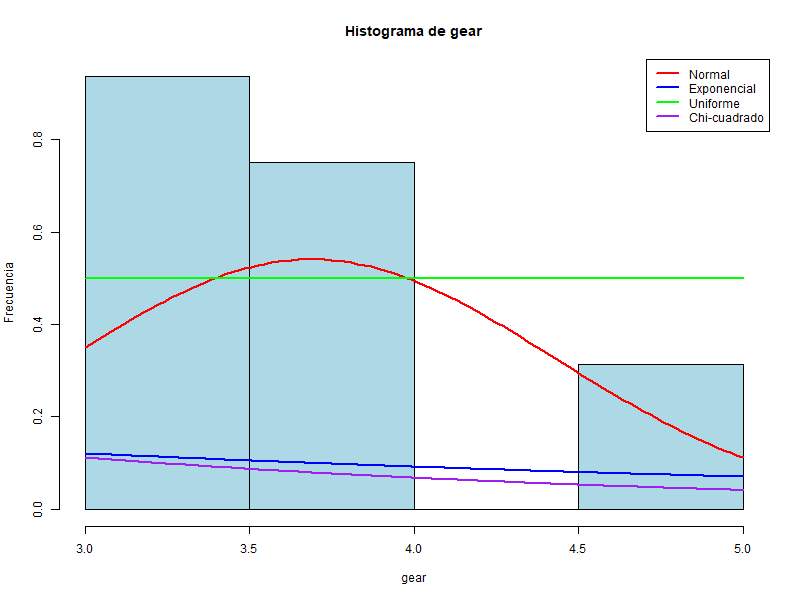
\includegraphics[width=0.5\textwidth]{Densidad/histograma_gear.png}
			\caption{Histograma para gear}
			\label{fig:histograma_gear}
			\vspace{0.5cm}
		\end{figure}

	\item \textbf{carb (Carburetors)}

	      \begin{itemize}
		      \item \textbf{Descripción:} Número de carburadores.
		      \item \textbf{Escala:} Cuantitativa Discreta.
		      \item \textbf{Significado:} Indica cuántos carburadores tiene el automóvil, lo que afecta la mezcla de aire y combustible y, por ende, el rendimiento del motor.
	      \end{itemize}

	      \begin{figure}[H]
		      \centering
		      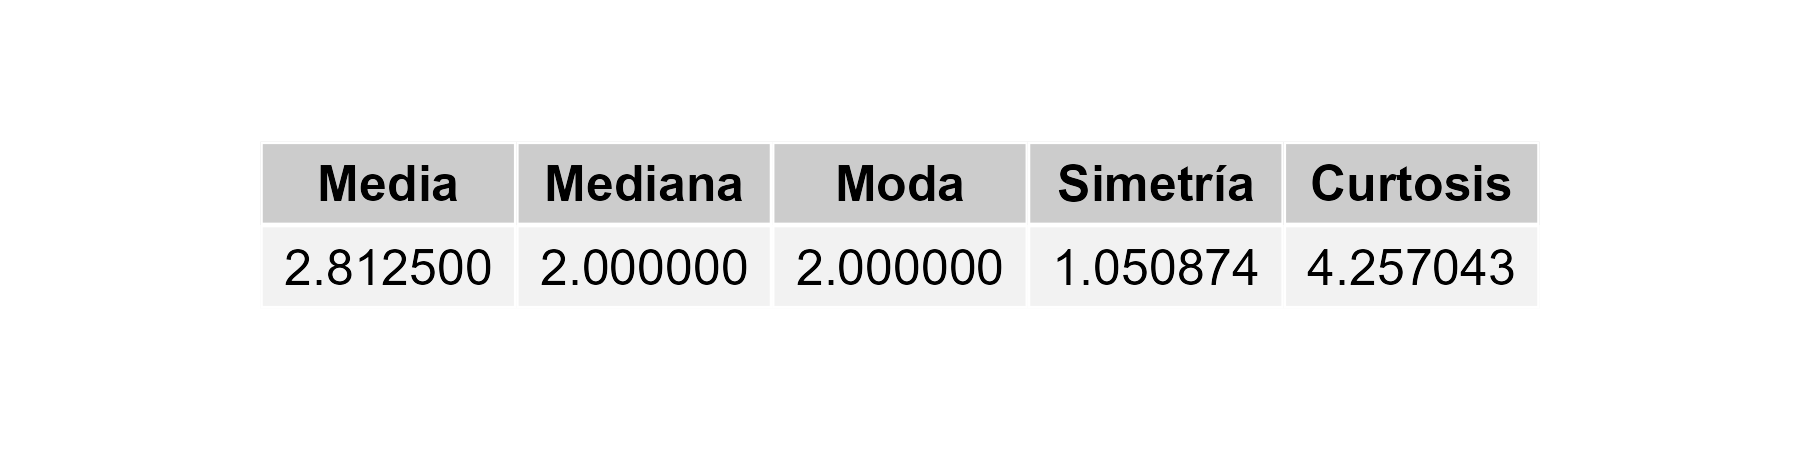
\includegraphics[width=0.8\textwidth]{MTC/carb_central.png}
		      \caption{Medidas de tendencia central para la variable \texttt{carb}.}
		      \label{fig:carb_central}
	      \end{figure}

	      \begin{figure}[H]
		      \centering
		      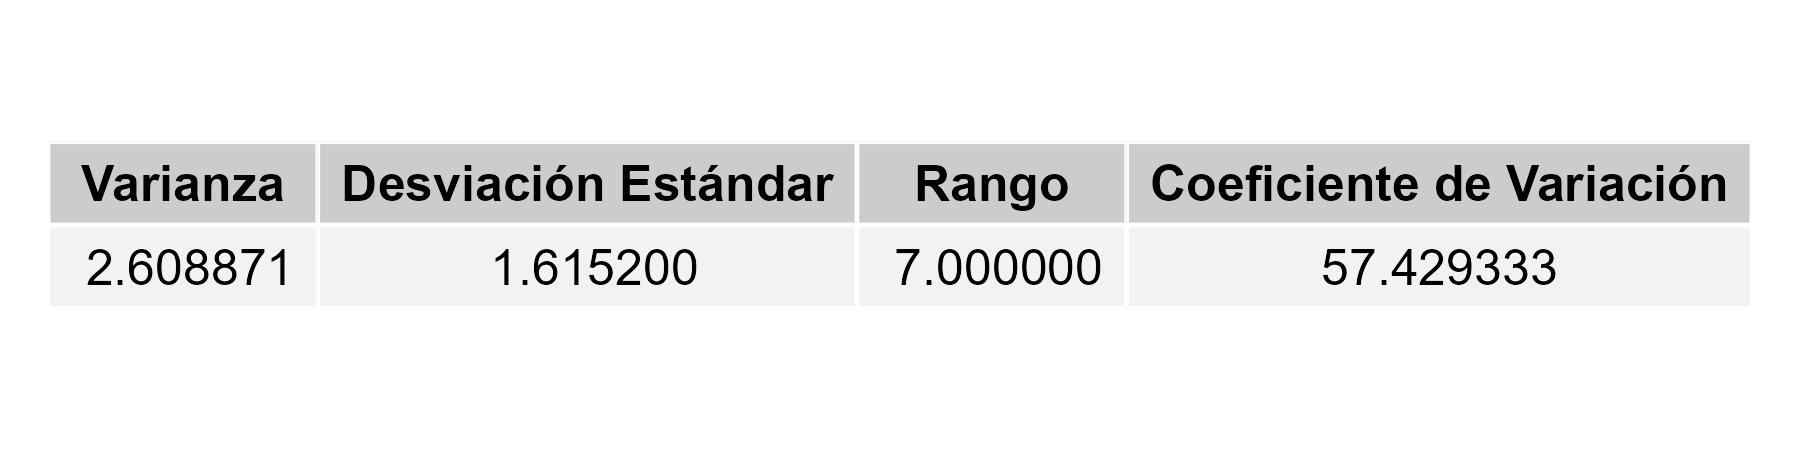
\includegraphics[width=0.8\textwidth]{MTC/carb_dispersion.png}
		      \caption{Medidas de dispersión para la variable \texttt{carb}.}
		      \label{fig:carb_dispersion}
	      \end{figure}
	    
	      \begin{itemize}
		      \item \textbf{Media:} El promedio es 2.81 carburadores, reflejando una moderada complejidad en los motores.
		      \item \textbf{Mediana:} El valor central es 2 carburadores.
		      \item \textbf{Moda:} La moda es 2 carburadores, indicando que es la configuración más común.
		      \item \textbf{Simetría:} Un valor de 1.05 indica una fuerte asimetría positiva, con algunos motores que tienen muchos carburadores.
		      \item \textbf{Curtosis:} Con 4.26, la distribución es leptocúrtica, con colas más pesadas.
		      \item \textbf{Varianza y Desviación Estándar:} La varianza de 2.61 y desviación estándar de 1.62 indican una dispersión significativa.
		      \item \textbf{Rango:} El rango de 7 carburadores muestra una gran diferencia en la complejidad de los motores.
		      \item \textbf{Coeficiente de Variación:} Con 57.43\%, existe una alta variabilidad relativa.
	      \end{itemize}

		  \begin{figure}[H]
			\centering
			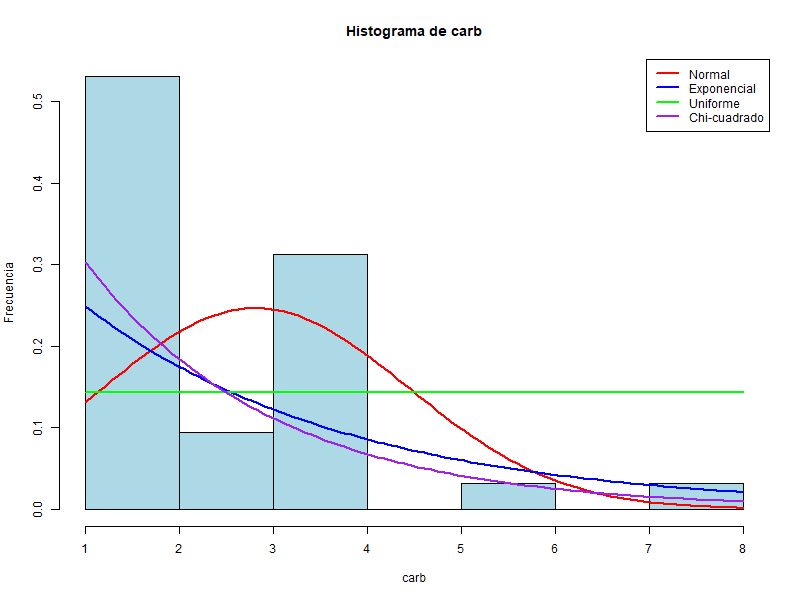
\includegraphics[width=0.5\textwidth]{Densidad/histograma_carb.png}
			\caption{Histograma para carb}
			\label{fig:histograma_carb}
			\vspace{0.5cm}
		\end{figure}

\end{enumerate}
En general, el análisis muestra que algunas variables, como \textit{mpg}, \textit{hp}, y \textit{disp}, presentan una alta dispersión y asimetría, lo que sugiere que los vehículos en el conjunto de datos tienen una gran diversidad en términos de eficiencia, potencia y tamaño del motor. Otras variables, como \textit{vs} y \textit{am}, son binarias, con poca variabilidad interna. El coeficiente de variación y la simetría son claves para entender cómo los datos están distribuidos y cómo pueden variar las características del vehículo.


\section{Resultados de la Matriz de Correlación}
A continuación se presentan algunos de los hallazgos clave de la matriz de correlación:

\begin{table}[h]
	\centering
	\begin{tabular}{lccccccccccc}
		\hline
		Variable & mpg   & cyl   & disp  & hp    & drat  & wt    & qsec  & vs    & am    & gear  & carb  \\ \hline
		mpg      & 1.00  & -0.85 & -0.87 & -0.77 & 0.68  & -0.87 & 0.74  & 0.66  & 0.60  & 0.48  & -0.55 \\
		cyl      & -0.85 & 1.00  & 0.90  & 0.78  & -0.50 & 0.87  & -0.59 & -0.81 & -0.52 & 0.36  & 0.55  \\
		disp     & -0.87 & 0.90  & 1.00  & 0.91  & -0.49 & 0.88  & -0.71 & -0.71 & -0.49 & 0.38  & 0.66  \\
		hp       & -0.77 & 0.78  & 0.91  & 1.00  & -0.25 & 0.66  & -0.66 & -0.55 & -0.68 & 0.43  & 0.66  \\
		drat     & 0.68  & -0.50 & -0.49 & -0.25 & 1.00  & -0.39 & 0.11  & 0.13  & 0.79  & 0.29  & -0.09 \\
		wt       & -0.87 & 0.87  & 0.88  & 0.66  & -0.39 & 1.00  & -0.70 & -0.55 & -0.58 & 0.30  & 0.43  \\
		qsec     & 0.74  & -0.59 & -0.71 & -0.66 & 0.11  & -0.70 & 1.00  & 0.74  & 0.59  & -0.17 & -0.55 \\
		vs       & 0.66  & -0.81 & -0.71 & -0.55 & 0.13  & -0.55 & 0.74  & 1.00  & 0.23  & 0.36  & -0.18 \\
		am       & 0.60  & -0.52 & -0.49 & -0.68 & 0.79  & -0.58 & 0.59  & 0.23  & 1.00  & 0.43  & -0.26 \\
		gear     & 0.48  & 0.36  & 0.38  & 0.43  & 0.29  & 0.30  & -0.17 & 0.36  & 0.43  & 1.00  & -0.12 \\
		carb     & -0.55 & 0.55  & 0.66  & 0.66  & -0.09 & 0.43  & -0.55 & -0.18 & -0.26 & -0.12 & 1.00  \\ \hline
	\end{tabular}
	\caption{Matriz de Correlación de las Variables del Dataset mtcars}
	\label{tab:correlation_matrix}
\end{table}

\begin{figure}[h] % 'h' indica que la imagen debe aparecer aquí
	\centering % Centra la imagen
	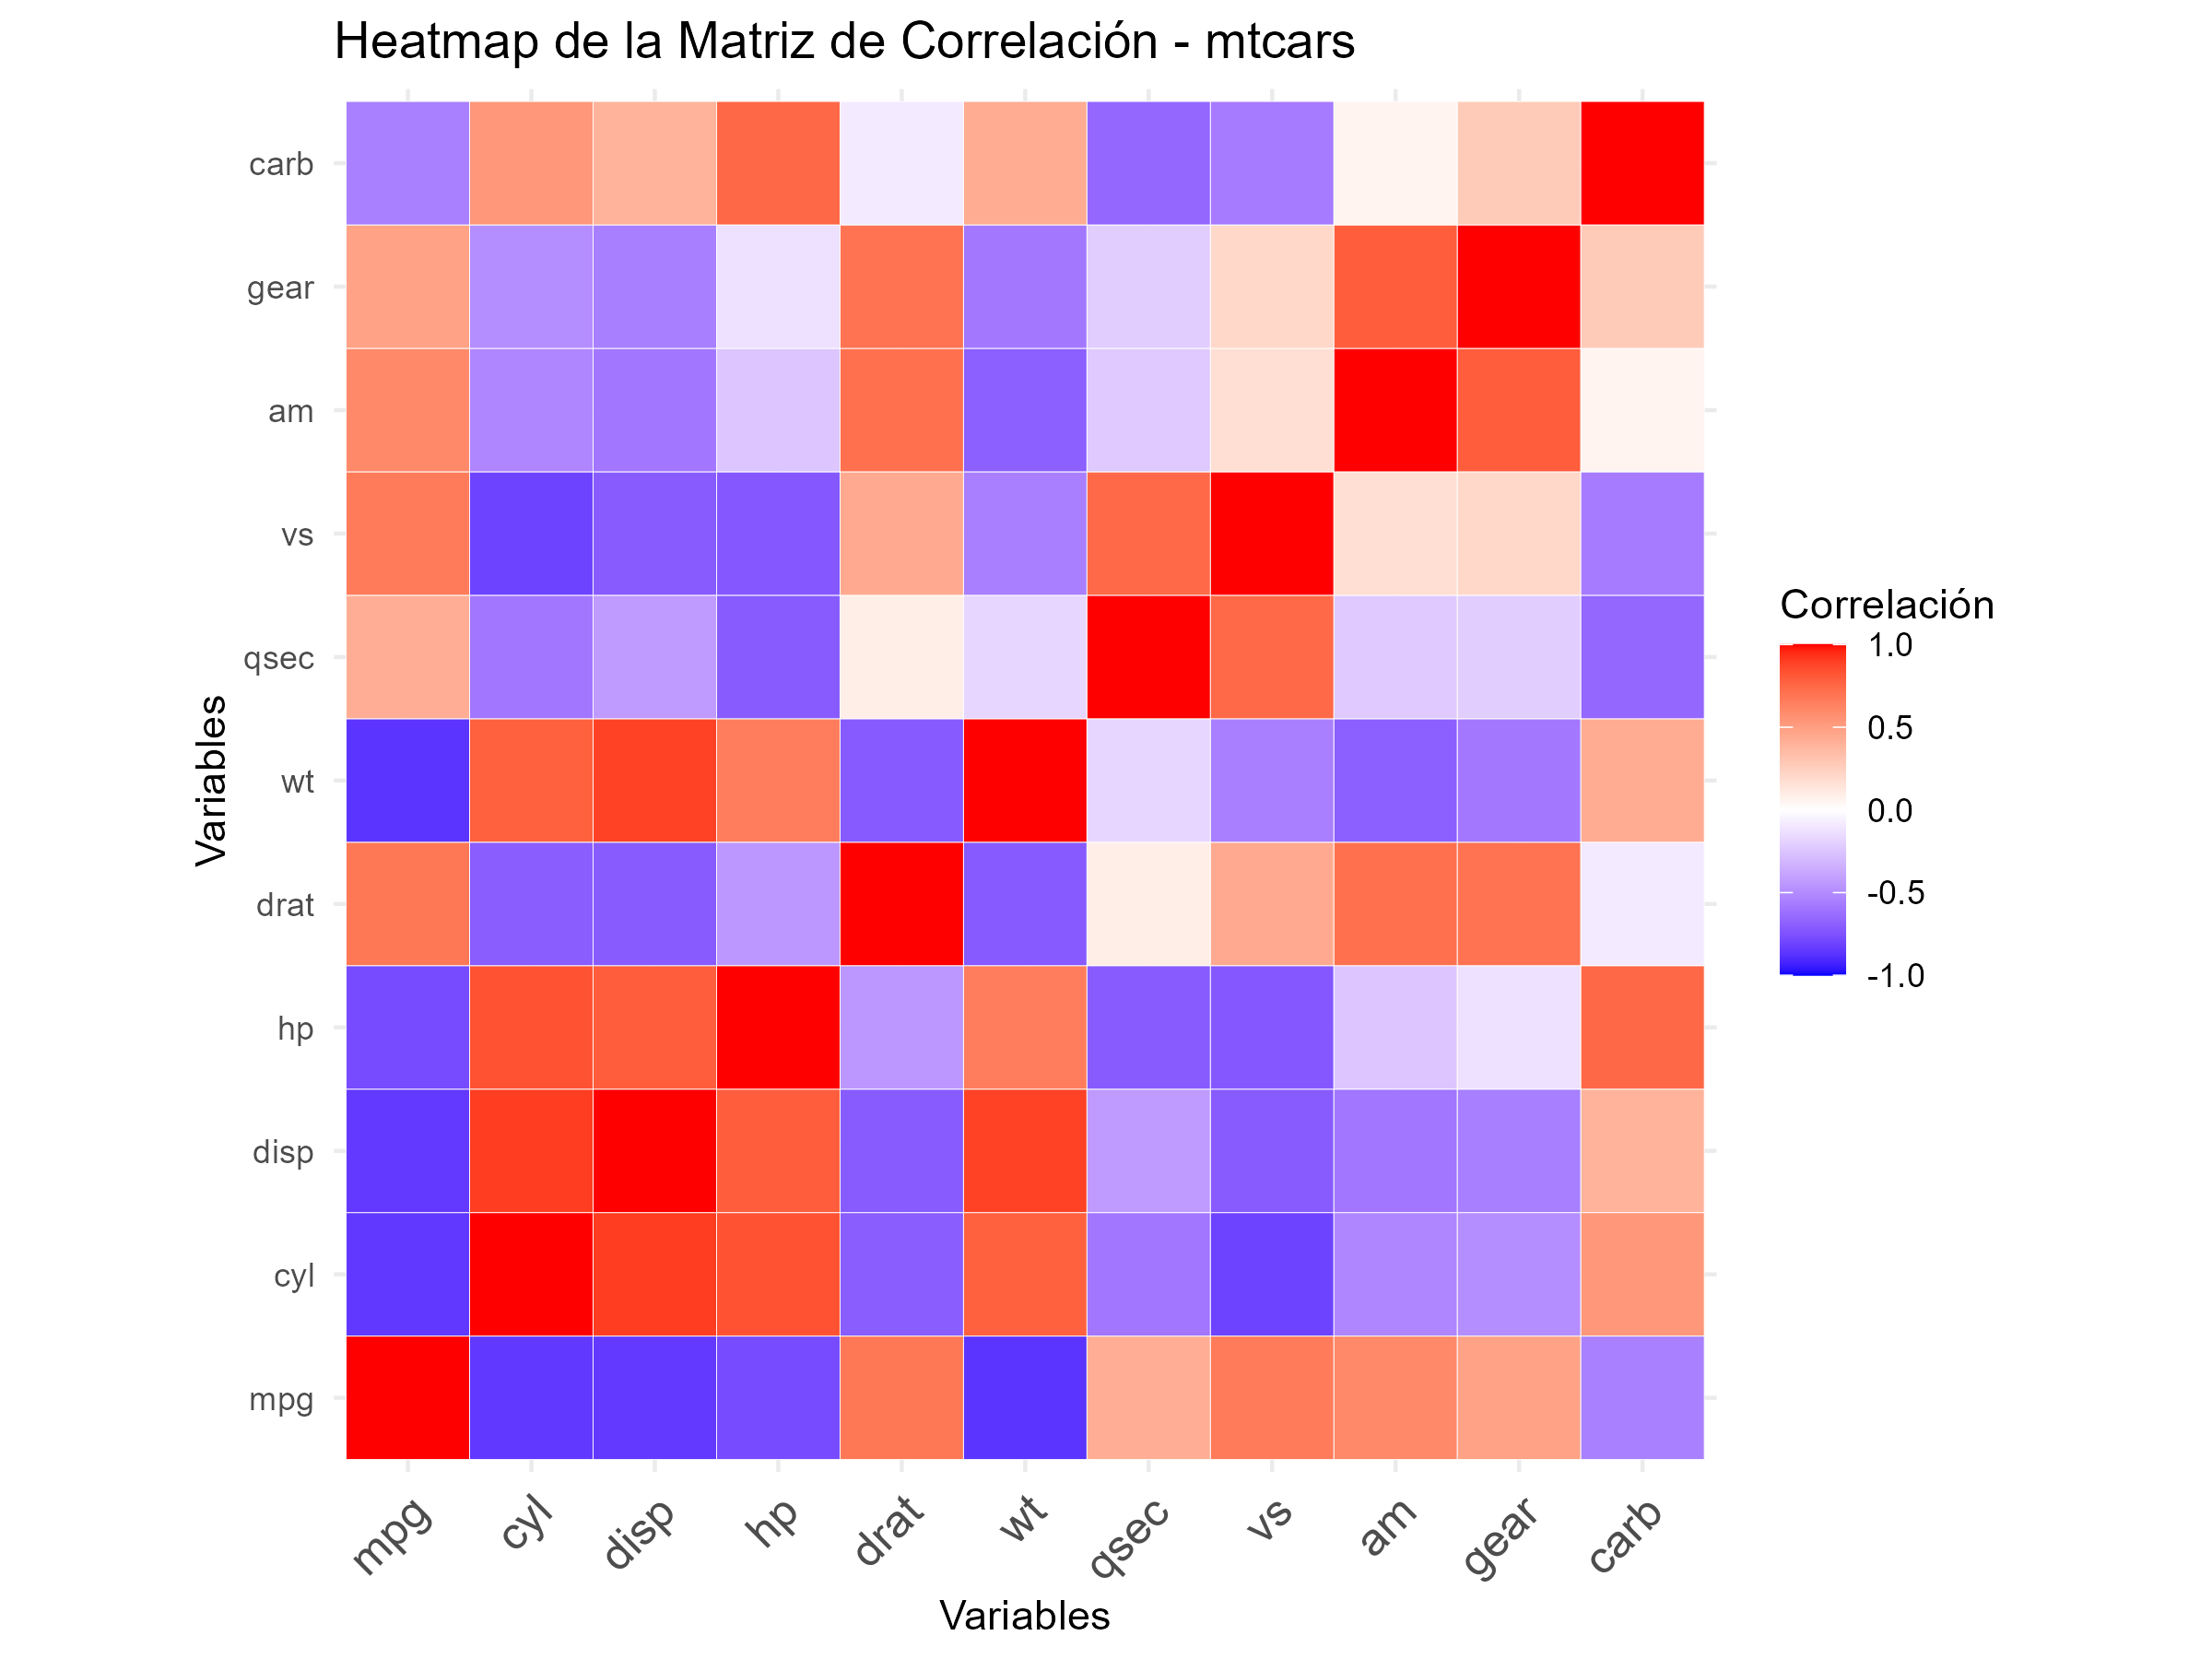
\includegraphics[width=0.8\textwidth]{heatmap_correlation_mtcars.png}
	\caption{Grafico de Calor , Correlaciones } % Título de la figura
	\label{fig:mi_imagen} % Etiqueta para referencias cruzadas
\end{figure}

\section{Resumen de Hallazgos}
\begin{itemize}
	\item \textbf{Correlaciones Fuertes}:
	      \begin{itemize}
		      \item \texttt{mpg} y \texttt{wt}: Correlación negativa fuerte (-0.87), indicando que a mayor peso del automóvil, menor es el rendimiento de combustible.
		      \item \texttt{mpg} y \texttt{cyl}: Correlación negativa fuerte (-0.85), sugiriendo que los automóviles con más cilindros tienden a tener un menor rendimiento de combustible.
		      \item \texttt{hp} y \texttt{disp}: Correlación positiva fuerte (0.91), indicando que a mayor desplazamiento del motor, mayor es la potencia en caballos de fuerza.
	      \end{itemize}
	      Lo que tambien es visible en los siguientes graficos de dispersion que relacionan ambas variables

	      \begin{figure}[H]
		      \centering
		      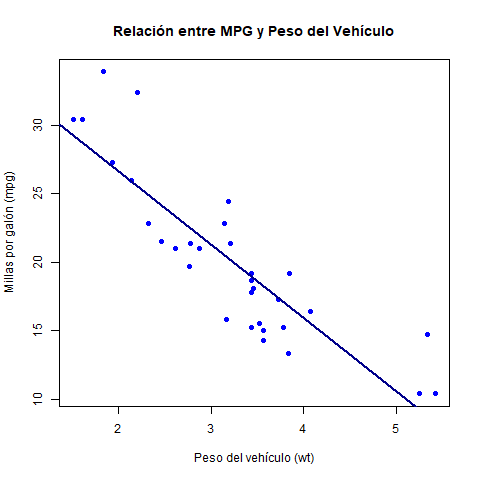
\includegraphics[width=0.5\textwidth]{mpg_vs_wt.png}
		      \label{fig:mpg_vs_wt}
		      \vspace{0.5cm} % Espacio entre las imágenes
	      \end{figure}

	      \begin{figure}[H]
		      \centering
		      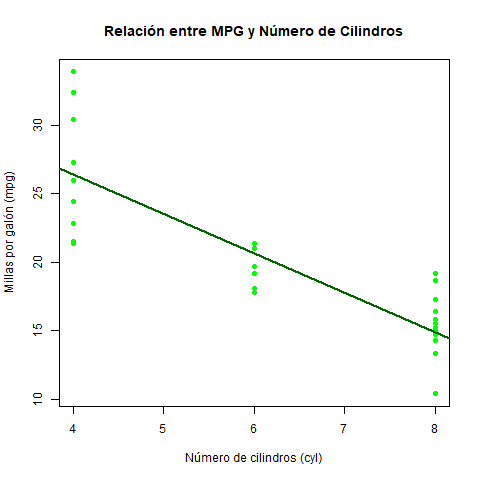
\includegraphics[width=0.5\textwidth]{mpg_vs_cyl.png}
		      \label{fig:mpg_vs_cyl}
		      \vspace{0.5cm} % Espacio entre las imágenes
	      \end{figure}

	      \begin{figure}[H]
		      \centering
		      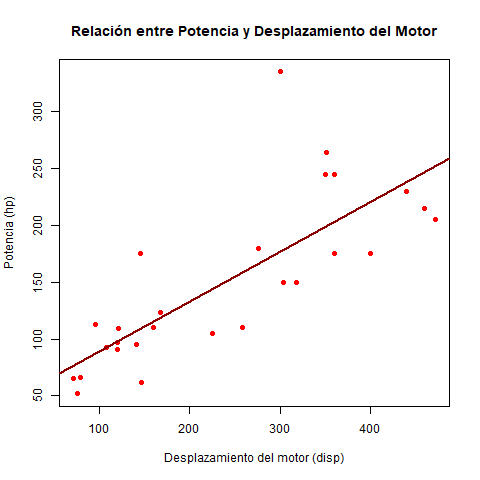
\includegraphics[width=0.5\textwidth]{hp_vs_disp.png}
		      \label{fig:hp_vs_disp}
		      \vspace{0.5cm} % Espacio entre las imágenes
	      \end{figure}

	\item \textbf{Correlaciones Moderadas}:
	      \begin{itemize}
		      \item \texttt{mpg} y \texttt{drat}: Correlación positiva moderada (0.68), sugiriendo que una mayor relación de transmisión puede estar asociada con un mejor rendimiento de combustible.
		      \item \texttt{am} y \texttt{mpg}: Correlación positiva moderada (0.60) entre el tipo de transmisión (manual) y el rendimiento de combustible.
	      \end{itemize}

	\item \textbf{Correlaciones Débiles}:
	      \begin{itemize}
		      \item \texttt{gear} y \texttt{mpg}: Correlación moderada (0.48), indicando que el número de marchas tiene un efecto, pero no tan fuerte como otras variables.La correlación moderada sugiere que el número de marchas puede influir en el rendimiento de combustible, pero no es el único factor. Es decir, un automóvil con más marchas podría tener un mejor rendimiento de combustible, pero hay otras variables (como el peso del automóvil, el tipo de motor, etc.) que también juegan un papel importante.
		      \item \texttt{drat} y \texttt{carb}: Correlación débil (-0.09), sugiriendo que no hay una relación significativa entre la relación de transmisión y el número de carburadores.
	      \end{itemize}
\end{itemize}

\section{Conclusiones}
El análisis de la matriz de correlación del conjunto de datos \texttt{mtcars} revela varias relaciones significativas entre las variables. Las correlaciones negativas entre el peso y el rendimiento de combustible, así como entre el número de cilindros y el rendimiento de combustible, son particularmente notables. Esto sugiere que los automóviles más pesados y aquellos con más cilindros tienden a ser menos eficientes en términos de consumo de combustible. Por otro lado, las correlaciones positivas entre el desplazamiento y la potencia sugieren que los motores más grandes tienden a ser más potentes.

Estos hallazgos son útiles para comprender cómo las características de los automóviles se relacionan entre sí y pueden guiar decisiones sobre el diseño y la selección de vehículos en función de su rendimiento y eficiencia.
\section{Analisis de la distribucion de Chi-Cuadrado}
En el dataset \texttt{mtcars}, las variables categóricas que pueden ser analizadas con la prueba Chi-Cuadrado son:
\begin{itemize}
    \item \texttt{vs}: Tipo de motor (0 = V-shaped, 1 = straight).
    \item \texttt{am}: Tipo de transmisión (0 = automática, 1 = manual).
    \item \texttt{gear}: Número de engranajes (3, 4, 5).
    \item \texttt{carb}: Número de carburadores (1, 2, 3, 4, 6, 8).
    \item \texttt{cyl}: Número de cilindros (4, 6, 8).
\end{itemize}

\begin{flushleft}
\textbf{Variables: \texttt{vs} y \texttt{am}}
\begin{itemize}
    \item $X^2 = 0.3475355$, $df = 1$, $p$-value = 0.5555115
    \item \textbf{Conclusión:} No hay evidencia de una relación significativa entre \texttt{vs} y \texttt{am}
\end{itemize}

\textbf{Variables: \texttt{vs} y \texttt{gear}}
\begin{itemize}
    \item $X^2 = 12.22434$, $df = 2$, $p$-value = 0.002215739
    \item \textbf{Conclusión:} Hay una relación significativa entre \texttt{vs} y \texttt{gear}
\end{itemize}

\textbf{Variables: \texttt{vs} y \texttt{carb}}
\begin{itemize}
    \item $X^2 = 15.33968$, $df = 5$, $p$-value = 0.009005379
    \item \textbf{Conclusión:} Hay una relación significativa entre \texttt{vs} y \texttt{carb}
\end{itemize}

\textbf{Variables: \texttt{vs} y \texttt{cyl}}
\begin{itemize}
    \item $X^2 = 21.33993$, $df = 2$, $p$-value = $2.323 \times 10^{-5}$
    \item \textbf{Conclusión:} Hay una relación significativa entre \texttt{vs} y \texttt{cyl}.
\end{itemize}

\textbf{Variables: \texttt{am} y \texttt{gear}}
\begin{itemize}
    \item $X^2 = 20.94467$, $df = 2$, $p$-value = $2.830889 \times 10^{-5}$
    \item \textbf{Conclusión:} Hay una relación significativa entre \texttt{am} y \texttt{gear}.
\end{itemize}

\textbf{Variables: \texttt{am} y \texttt{carb}}
\begin{itemize}
    \item $X^2 = 6.237131$, $df = 5$, $p$-value = 0.2838241
    \item \textbf{Conclusión:} No hay evidencia de una relación significativa entre \texttt{am} y \texttt{carb}
\end{itemize}

\textbf{Variables: \texttt{am} y \texttt{cyl}}
\begin{itemize}
    \item $X^2 = 8.740733$, $df = 2$, $p$-value = 0.01264661
    \item \textbf{Conclusión:} Hay una relación significativa entre \texttt{am} y \texttt{cyl}
\end{itemize}

\textbf{Variables: \texttt{gear} y \texttt{carb}}
\begin{itemize}
    \item $X^2 = 16.5181$, $df = 10$, $p$-value = 0.08573092
    \item \textbf{Conclusión:} No hay evidencia de una relación significativa entre \texttt{gear} y \texttt{carb}
\end{itemize}

\textbf{Variables: \texttt{gear} y \texttt{cyl}}
\begin{itemize}
    \item $X^2 = 18.03636$, $df = 4$, $p$-value = 0.001214066
    \item \textbf{Conclusión:} Hay una relación significativa entre \texttt{gear} y \texttt{cyl}
\end{itemize}

\textbf{Variables: \texttt{carb} y \texttt{cyl}}
\begin{itemize}
    \item $X^2 = 24.38887$, $df = 10$, $p$-value = 0.006632478
    \item \textbf{Conclusión:} Hay una relación significativa entre \texttt{carb} y \texttt{cyl}
\end{itemize}
\end{flushleft}

Este análisis es útil para entender cómo las diferentes características de los automóviles en el dataset \texttt{mtcars} están asociadas entre sí. Variables como el tipo de motor (\texttt{vs}), el tipo de transmisión (\texttt{am}), y el número de cilindros (\texttt{cyl}) muestran dependencias importantes que podrían ser exploradas más a fondo en estudios adicionales.

\section{Descripción del Gráfico}
\begin{figure}[H] % 'h' indica que la imagen debe aparecer aquí
	\centering % Centra la imagen
	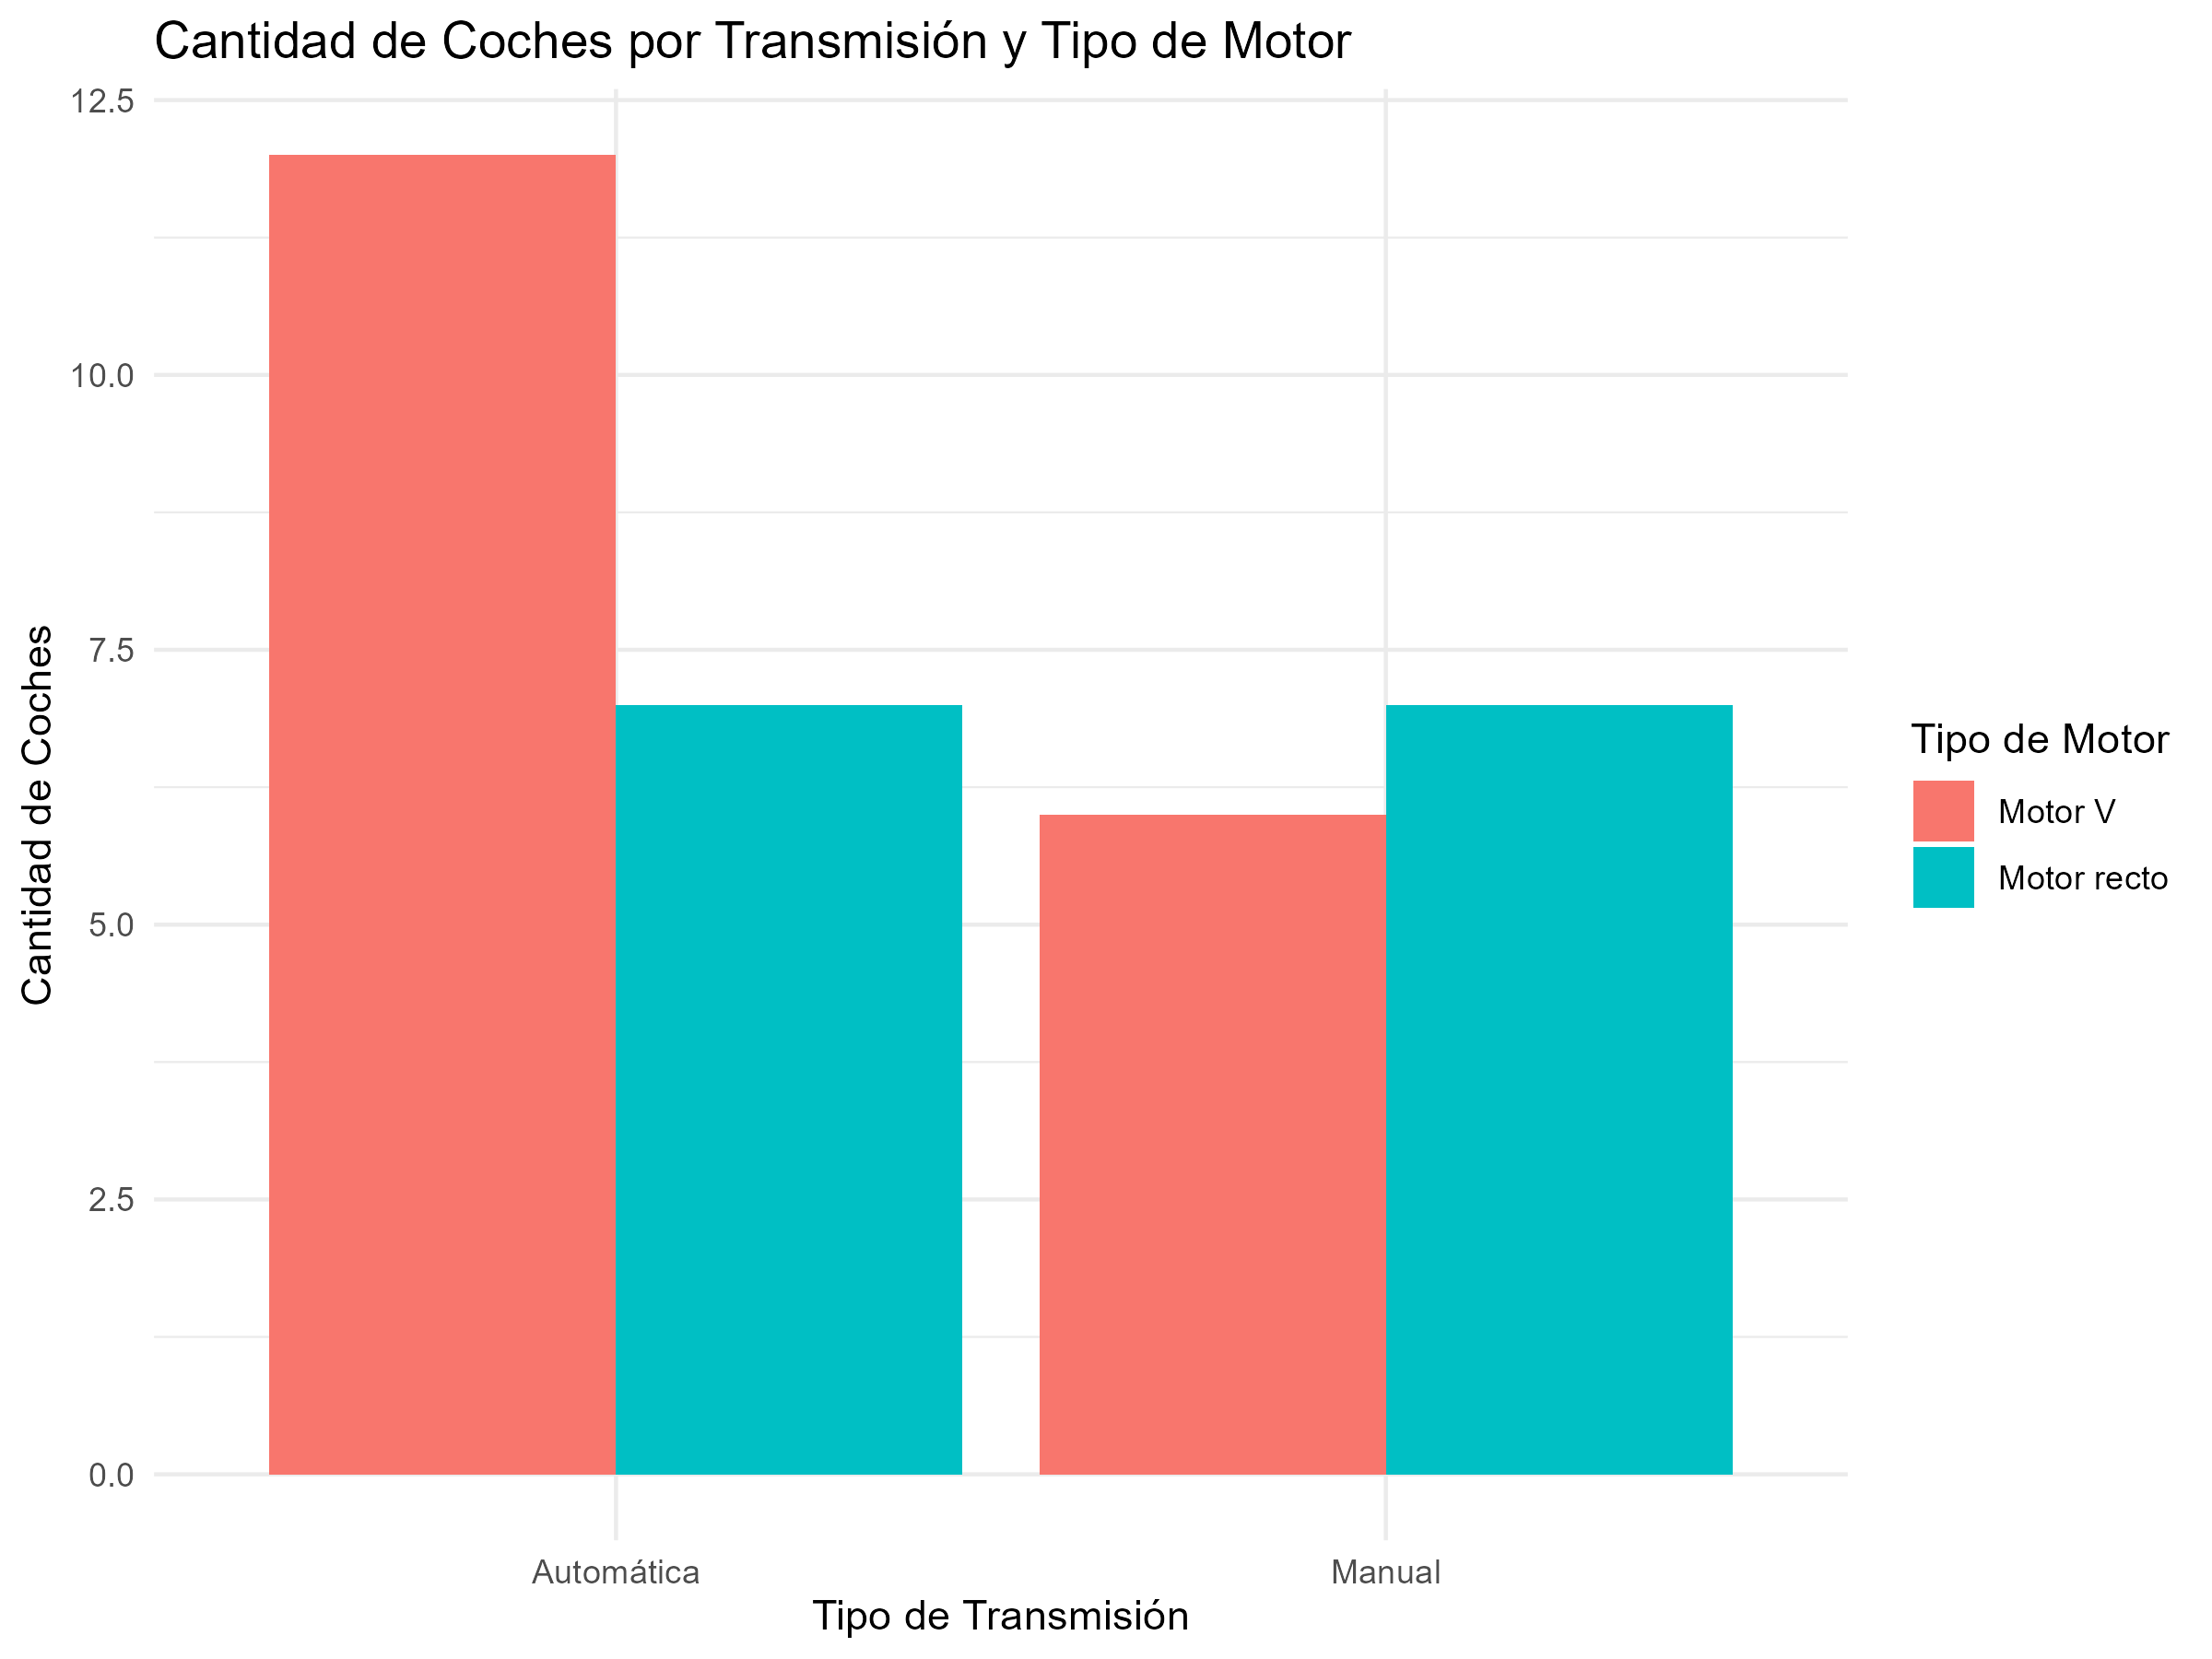
\includegraphics[width=0.8\textwidth]{mtcars_transmision_motor.png}
	\caption{Grafico de Barras, Distribucion Chi-Cuadrado} % Título de la figura
	\label{fig:mi_imagen} % Etiqueta para referencias cruzadas
\end{figure}

\subsection{Ejes del Gráfico}
\begin{itemize}
	\item \textbf{Eje X (Tipo de Transmisión)}: Este eje representa el tipo de transmisión de los automóviles, donde:
	      \begin{itemize}
		      \item 0 representa transmisión automática.
		      \item 1 representa transmisión manual.
	      \end{itemize}
	\item \textbf{Eje Y (Frecuencia)}: Este eje muestra la frecuencia observada de automóviles para cada combinación de tipo de transmisión y tipo de motor.
\end{itemize}

\subsection{Barras}
\begin{itemize}
	\item Cada barra representa la frecuencia de automóviles que tienen una combinación específica de tipo de transmisión y tipo de motor.
	\item Las barras están agrupadas por el tipo de transmisión (automática y manual) y se diferencian por color según el tipo de motor:
	      \begin{itemize}
		      \item 0 representa un motor en línea.
		      \item 1 representa un motor en V.
	      \end{itemize}
\end{itemize}

\subsection{Colores}
Los colores de las barras indican el tipo de motor. Esto permite una comparación visual rápida entre las frecuencias de los diferentes tipos de motores para cada tipo de transmisión.

\section{Análisis del Gráfico}

\subsection{Comparación de Frecuencias}
Al observar las alturas de las barras, puedes comparar cuántos automóviles tienen transmisión automática frente a manual para cada tipo de motor. Por ejemplo, si la barra para transmisión manual y motor en línea es más alta que la de transmisión automática y motor en línea, esto indica que hay más automóviles con transmisión manual que automática en esa categoría.

\subsection{Tendencias Observadas}
Puedes identificar tendencias en la distribución de los tipos de transmisión y motor. Por ejemplo:
\begin{itemize}
	\item Si hay más automóviles con transmisión manual que automática para ambos tipos de motor, esto podría sugerir una preferencia por la transmisión manual en el conjunto de datos.
	\item Si la frecuencia de motores en línea es mayor en un tipo de transmisión en comparación con el otro, esto puede indicar una relación entre el tipo de transmisión y el tipo de motor.
\end{itemize}

\subsection{Relación entre Variables}
El gráfico permite evaluar visualmente si existe una relación entre el tipo de transmisión y el tipo de motor. Si las frecuencias son muy diferentes entre las combinaciones, esto sugiere que podría haber una asociación significativa entre estas variables. Si las frecuencias son similares, podría indicar que el tipo de transmisión no está relacionado con el tipo de motor.
\begin{itemize}
    \item \textbf{Comparación entre transmisiones y motores:}
    \begin{itemize}
        \item \textbf{Coches automáticos:} La mayoría tiene motor en V, mientras que una minoría tiene motor recto, lo que es visible pues la barra de color naranja que representa los motores en V es mayor que la barra de color azul, que es la de los motores rectos.
        \item \textbf{Coches manuales:} Los coches con transmisión manual están equilibrados entre motor en V y motor recto, pues como es visible ambas barras tienen tamaño similar.
    \end{itemize}

    \item \textbf{Conclusión general:} 
    El número de coches con transmisión automática es menor que el de coches con transmisión manual. Además, se observa una preferencia por motores en V en los coches automáticos, mientras que los coches con transmisión manual muestran una distribución más equilibrada entre motores en V y rectos.
\end{itemize}

\end{document}
